%\documentclass[]{dinel-upm}
\documentclass[a4paper,12pt]{report}
%\setlength{\columnsep}{0.7cm} % space between columns
\usepackage{filecontents}
\usepackage{gensymb}


\usepackage{lipsum}
\usepackage{fancyhdr}
\usepackage{titlesec}
\usepackage[spanish,es-tabla]{babel}
\usepackage[utf8]{inputenc}
\usepackage{amsmath,amssymb,amsthm}
\usepackage{afterpage}
\usepackage[left=2.5cm,right=2.5cm,top=2.5cm,bottom=2.5cm]{geometry}
\usepackage{tocloft}
\usepackage{enumerate} 
\usepackage{tikz}
\usetikzlibrary{shapes,arrows}

\usepackage{wrapfig}
\usepackage{graphicx,tabularx}
\usepackage{eurosym}
\usepackage{multicol}
\usepackage{multirow}
\usepackage{rotating}
%\usepackage{pdfpages}
\usepackage{pdflscape}
\usepackage{booktabs}
\usepackage[hyphens]{url}
\usepackage[document]{ragged2e}
\usepackage{caption}
\DeclareCaptionListFormat{myfmt}{#1.#2}
\usepackage[list=true,listformat=myfmt]{subcaption}

%\usepackage{tikz}
\usepackage[cuteinductors,americanvoltages,americancurrents,american]{circuitikz}

\newcommand{\newItemUrl}[1]{\href{#1}{#1}}
\newcommand{\tabitem}{~~\llap{--}~~}
\newcommand{\newItem}[1]{\multicolumn{3}{|p{11cm}|}{\tabitem #1}\\}

\newcommand\Tstrut{\rule{0pt}{2.6ex}} 
\newcommand\Zstrut{\rule{0pt}{3.2ex}} 
\newcommand\Bstrut{\rule[-0.9ex]{0pt}{0pt}}
\newcommand{\HRule}{\rule{\textwidth}{0.1mm}} 		
\usepackage{hyperref}
					% horizontal line and its thickness


\titleformat
{\chapter} % command
[hang] % shape
{  \normalfont\bfseries\Huge} % format
{} % label
{0.5ex} % sep
{
%	\centering 
} % before-code
[] % after-code


%nuevo comando

\newcommand{\tb}[1]{\textcolor{blue}{#1}}
\usepackage[english]{cleveref} %con este paquete si usas \cref{label} te pone automáticamente figura,ecuacion..

\newcommand{\refAnexo}[1]{(Anexo \ref{#1})}
\newcommand{\refFigura}[1]{(Figura \ref{#1})}
\newcommand{\refApartado}[1]{(Apartado \ref{#1})}

%\title{\textbf{Control de drones mediante Reinforcement Learning en plataformas reales}}
%\title{\textbf{Plataforma hardware y software para el desarrollo y validación de algoritmos de control de actitud para cuadricópteros}}
\title{\textbf{Kit de desarrollo y validación de algoritmos de control de actitud para cuadricópteros}}

\author{Miguel Fernández Cortizas}
\date{}

\newcommand{\grad}{$^{\circ}$}


\usepackage{dtk-logos} % for BibTeX stylized logo
\usetikzlibrary{babel}
\usepackage{tikz}
\usetikzlibrary{matrix,chains,positioning,decorations.pathreplacing,arrows}

\usepackage{pgfplots}
\usepackage{ifthen}

\usepackage{amsmath}
\DeclareMathOperator{\sigm}{sigm}
\newcommand{\diff}{\mathop{}\!\mathrm{d}}


\begin{document}
	\maketitle
	
	\abstract
hola
	
	\tableofcontents

	\justify
	
	\usetikzlibrary{shapes,arrows,positioning,calc,chains,scopes}

% colors
\definecolor{snowymint}{HTML}{E3F8D1}
\definecolor{wepeep}{HTML}{FAD2D2}
\definecolor{portafino}{HTML}{F5EE9D}
\definecolor{plum}{HTML}{DCACEF}
\definecolor{sail}{HTML}{A3CEEE}
\definecolor{highland}{HTML}{6D885A}

\tikzstyle{signal}=[arrows={-latex},draw=black,line width=1.5pt,rounded corners=4pt]

% RNN
\tikzstyle{block}=[draw=black,line width=1.0pt]
\tikzstyle{cell}=[style=block,draw=highland,fill=snowymint,
    rounded corners]
\tikzstyle{celllayer}=[style=block,draw,fill=portafino,
    inner sep=1pt,outer sep=0,
    minimum width=28pt, minimum height=14pt]
\tikzstyle{pointwise}=[style=block,ellipse,fill=wepeep,
    inner sep=1pt,outer sep=0, minimum size=12pt]

\def\iolen{24pt}
\def\intergape{2pt}

% MLP and CNN
\tikzstyle{netnode}=[circle, inner sep=0pt, text width=22pt, align=center, line width=1.0pt]
\tikzstyle{inputnode}=[netnode, fill=sail,draw=black]
\tikzstyle{hiddennode}=[netnode, fill=snowymint,draw=black]
\tikzstyle{outputnode}=[netnode, fill=plum,draw=black]

% Architecture
\def\layerwidth{90pt}
\def\layerheight{14pt}

\tikzstyle{layer}=[style=block, draw, fill=black!20!white,
    inner sep=1pt,outer sep=0, font=\footnotesize,
    text centered, 
    minimum width=\layerwidth, minimum height=\layerheight]

\tikzstyle{fc}=[style=layer, fill=blue!30!white]
\tikzstyle{conv}=[style=layer, fill=green!30!white]
\tikzstyle{activation}=[style=layer, fill=orange!30!white]
\tikzstyle{pool}=[style=layer, fill=red!30!white]
\tikzstyle{bn}=[style=layer, fill=cyan!30!white]
\tikzstyle{recurrent}=[style=layer, fill=purple!30!white]
\tikzstyle{softmax}=[style=layer, fill=yellow!30!white]
\tikzstyle{point}=[]
\tikzstyle{branch}=[coordinate]

\def\vlayerwidth{30pt}
\def\vlayerheight{3pt}
\def\vblockheight{28pt}

\tikzstyle{vlayer}=[minimum width=\vlayerwidth, minimum height=\vlayerheight]
\tikzstyle{vblock}=[minimum width=\vlayerwidth, minimum height=\vblockheight, text width=1cm, align=center]


% Precision, Recall
\colorlet{fn}{gray!90!green!30!white}
\colorlet{tp}{green!40!white}
\colorlet{fp}{red!40!white}
\colorlet{tn}{gray!90!red!20!white}

	\chapter*{Introducción}

	\chapter{Estado del arte}

El desarrollo del trabajo realizado se puede subdividir en dos campos: la construcción de la plataforma de sujeción del cuadricóptero y la experimentación con nuevos algoritmos de control empleando técnicas de aprendizaje por refuerzo. Es por esto que, con el ánimo de contextualizar este trabajo dentro de estos dos campos, se ha tratado el estado del arte de forma separada.

\section{Plataformas de control de cuadricópteros}

Debido a la creciente popularidad de estas aeronaves, muchas líneas de investigación han trabajado en probar y desarrollar distintos algoritmos de control, para comparar el rendimiento entre ellos. Para poder testear estos algoritmos es muy conveniente contar con una plataforma de control, que te permita medir el rendimiento de estos algoritmos de control de forma precisa y segura.

Principalmente, existen 2 tipos de plataformas para esté propósito: Plataformas tipo gimbal y estructuras con unión esférica. A continuación se tratará mas detalladamente las características de estas estructuras:

\subsection{Plataformas tipo gimbal}

Estas plataformas están formados por 3 anillos unidos entre ellos dos a dos, de tal forma que el anillo interior gira respecto al anillo que lo rodea y éste a su vez gira sobre el anillo exterior, como se puede observar en la figura \ref{gimbal}

\begin{figure}[htb!]
	\centering
	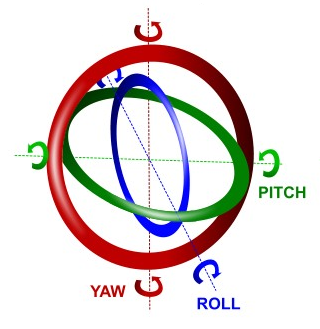
\includegraphics[width=0.42\textwidth]{estadodelarte/gimbal}
	\caption{Esquema estructura gimbal}
	\label{gimbal}
\end{figure}

Estas plataformas permiten que la aeronave gire entorno a su centro de gravedad, por lo que se reduce la influencia del peso de la aeronave en el control. Además es posible medir los ángulos de euler de la aeronave de forma directa empleando encoders en los ejes de rotación.

Hay empresas que están empezando a comercializar estas plataformas, tanto orientadas para la labor investigadora en el campo de los cuadricópteros , como para la labor docente que se puede llevar a cabo empleando estas plataformas con ánimo didáctico, para el aprendizaje de algoritmos de control. 

En cuanto a las  plataformas orientadas a la investigación, se encuentra la plataforma FFT gyro , desarrollada por Eureka Dynamics.

\begin{figure}[htb!]
	\centering
	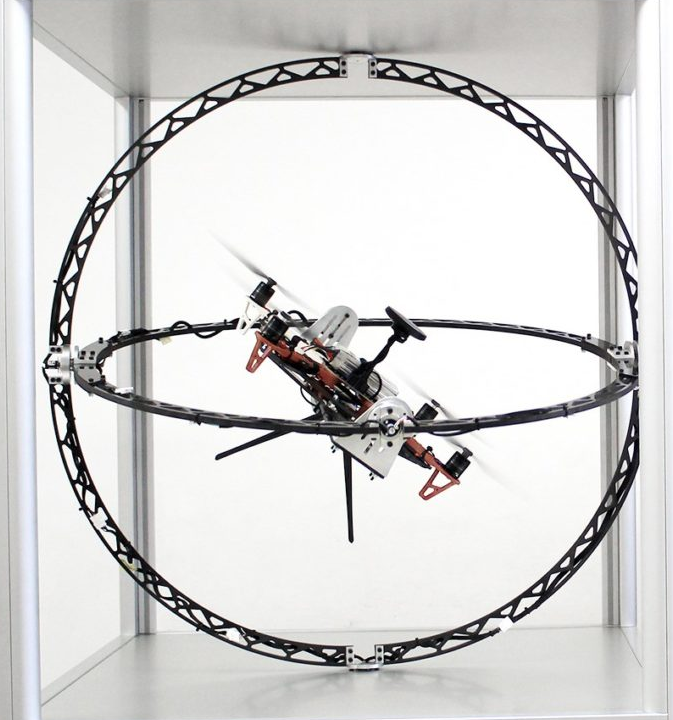
\includegraphics[width=0.6\textwidth]{estadodelarte/fft_gyro}
	\caption{Plataforma FFT Gyro de Eureka Dynamics}
	\label{giro_fft}
\end{figure}

Esta plataforma cuenta con encoders en cada eje de rotación para poder monitorizar el estado de la aeronave con gran precisión y esta construida en fibra de carbono para maximizar la rigidez de la estructura minimizando el peso.

\subsection{Plataformas con unión esférica}

Estas plataformas se unen a la aeronave a través de una unión esférica, la cual permite que el cuadricóptero pueda girar en tres ángulos, con algunas limitaciones. Por ejemplo, aunque en guiñada la aeronave pueda girar libremente, en alabeo y cabeceo este movimiento se ve restringido por las limitaciones mecánicas de la unión, véase \cref{union esferica}. Esto es una gran diferencia con respecto a las plataformas de tipo gimbal, en las que este suceso no ocurre, dado que en sus articulaciones no existen restricciones en los ángulos de giro.

A pesar de esto, estas plataformas condensan todos los giros en un único punto, por lo que el tamaño de la estructura requerida para anclar un cuadricóptero, es significativamente menor  que si se emplea una estructura de tipo gimbal.

\begin{figure}[htb!]
	\centering
	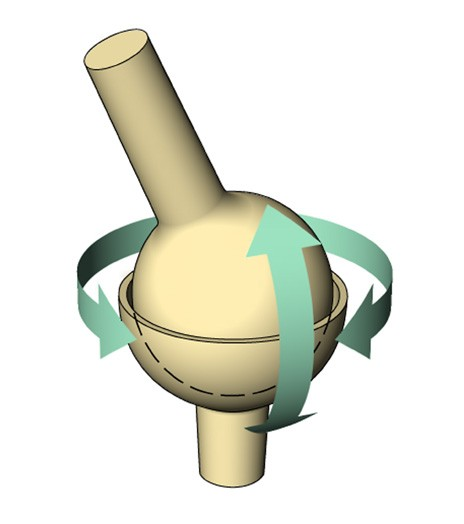
\includegraphics[width=0.4\textwidth]{estadodelarte/union_esferica}
	\caption{Esquema de una union esférica}
	\label{union esferica}
\end{figure}
\newpage
En cuanto a plataformas comerciales de esté tipo, cabe destacar las producidas por la empresa Quanser, la cuál ha desarrollado una plataforma con fines educativos, que emplea esta unión. Esta plataforma cuenta, al igual que la FFT Gyro con encoders, con la finalidad de conocer con precisión el estado de la aeronave.
   
\begin{figure}[htb!]
	\centering
	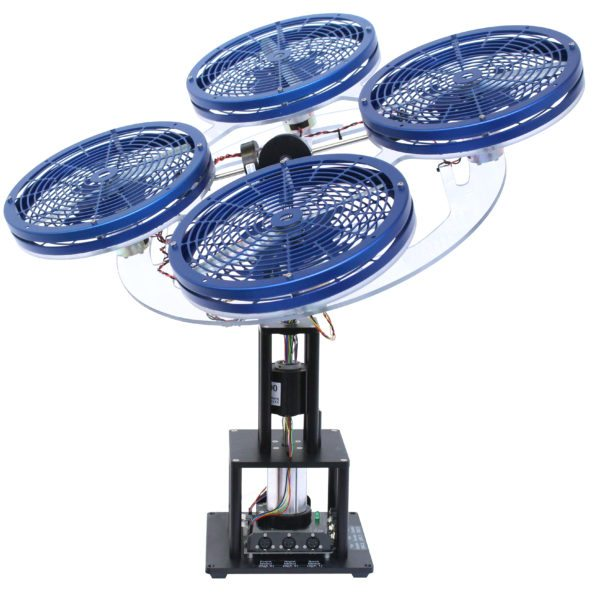
\includegraphics[width=0.5\textwidth]{estadodelarte/quanser}
	\caption{Plataforma 3 DOF Hover de la empresa Quanser}
	\label{union esferica}
\end{figure}

Entre las dos posibilidades, se ha optado por realizar una plataforma con una unión esférica debido a la mayor simplicidad y menor tamaño de este tipo de plataformas frente a su alternativa.
\section{Aprendizaje por refuerzo}
El aprendizaje por refuerzo o \textit{reinforcement learning} es una rama del aprendizaje automático en  la que un agente aprende a actuar a medida que va interactuando con su entorno. Es decir, el agente comienza realizando acciones aleatorias y va aprendiendo por ensayo-error. Para que el agente tenga noción de que acciones están ``bien'' y cuales no, el entorno proporciona una recompensa al agente en función de su comportamiento. Esta rama del aprendizaje automático se inspira en la psicología conductista.

Debido a esta capacidad de aprender de forma autónoma, sin necesidad de un conjunto previo de datos etiquetados, sino extrayendo información únicamente de su interacción con el entorno, estos algoritmos son muy empleados en el campo de la robótica para llevar a cabo tareas complicadas, tales como, aprender a andar o a manipular un cubo con destreza \cite{andrychowicz2018learning}.

Aunque existen una gran cantidad de ejemplos de uso de estas técnicas de aprendizaje en el ámbito de la robótica, en este trabajo se ha centrado en el empleo de estas técnicas al control de UAVs.

Los primeros experimentos en la utilización de algoritmos de control para UAVs, entrenados con aprendizaje con refuerzo, se llevaron a cabo con helicópteros. En 2004, HJ Kim et al. \cite{kim2004autonomous} emplearon algoritmos de \textit{reinforcement learning} para estabilizar (\textit{hover}) un helicóptero y conseguir realizar maniobras acrobáticas, para ello desarrollaron el algoritmo Pegasus \cite{ng2000pegasus}. Años después, en 2006 Andrew Y. et al \cite{ng2006autonomous} continuaron la investigación, en esta ocasión emplearon algoritmos que aprendían a realizar maniobras acrobáticas complejas, como mantener invertido al helicóptero. Para ello, realizaron un modelo estocástico no lineal de la dinámica del helicóptero, para, posteriormente, emplear ese modelo en simulación con el ánimo de generar un controlador capaz de estabilizar al helicóptero invertido.

En 2010 Travis Dierks et al. \cite{dierks2010output} desarrollaron un controlador no lineal, basado en redes neuronales, para estabilizar un cuadricóptero y seguir trayectorias. Para obtener un modelo completo de la aeronave, que fuera capaz también de tener en cuenta otros parámetros externos a la aeronave, como el coeficiente aerodinámico, el aprendizaje de la red neuronal se realizaba a tiempo real, mientras el cuadricóptero volaba. 

Unos años después, en 2017 Jemin Hwangbo et al. \cite{hwangbo2017control} desarrollaron un método para controlar un cuadricóptero con una red neuronal usando técnicas de \textit{reinforcement learning}. Desarrollaron un algoritmo, basado en la optimización determinista de la política y empleando descenso de gradientes natural para optimizar la misma. Consiguieron que el cuadricóptero fuera capaz de estabilizarse aún cuando partía de condiciones adversas, como ser lanzado casi boca abajo contra el suelo. Sin embargo, para conseguirlo, necesitaban frecuencias de actualización muy elevadas, del orden de los 100Khz, dos órdenes de magnitud mayor que un algoritmo típico.

 En 2018 William Koch et al. \cite{koch2019reinforcement} desarrollaron un entorno de simulación, GYMFC, para el desarrollo de nuevos algoritmos de control basados en redes neuronales. En su artículo compararon el rendimiento, en simulación, de distintos algoritmos de aprendizaje por refuerzo a la hora de cerrar el bucle de control en velocidad de un cuadricóptero. Posteriormente, a comienzos de 2019, desarrollaron Neuroflight \cite{koch2019neuroflight}, un \textit{firmware} para autopilotos \textit{open-source}. Este \textit{firmware}, a diferencia del de los autopilotos convencionales emplea bucles de control desarrollados con técnicas de aprendizaje por refuerzo, con los que consiguen controlar un cuadricóptero real. 

 
	\chapter{Fundamentos teóricos}

%\section{Control clásico}


%Una vez conseguida una estimación del estado en el instante $t$ ,  $S_t$ se necesita emplear un algoritmo de control que genere	las acciones $A_t$ correspondientes para llegar al estado $S_{t'}$ deseado de forma óptima.

%\tb{BUCLE DE CONTROL}


%Existe una gran cantidad de controladores clásicos que se pueden emplear para generar estos comandos, por ejemplo: PID o LQR.
%En este trabajo se han explorado 2 controladores: el primero de ellos se trata de un controlador clásico PID y el segundo consiste en un controlador no lineal modelizado por una red neuronal.

\section{Controlador PID}

Un regulador PID es un controlador lineal realimentado. Matemáticamente se expresa como 
\begin{equation}
	u(t) = \overbrace{\raisebox{0ex}[2.2\height]{$K_p e(t)$}}^\text{P} +\overbrace{K_i \int_{0}^{t}e(\tau)d\tau}^\text{I} + \overbrace{ K_d \frac{de(t)}{dt}}^\text{D}\;
\end{equation}

donde $e(t)$ es la señal de control, $u(t)$ representa la salida del regulador y $K_p,K_i,K_d$ son parámetros ajustables de los cuales depende la dinámica y la estabilidad del sistema. Como se puede observar, el regulador consta de tres partes: la parte proporcional (P) tiene en cuenta el error actual, la parte integral (I) tiene en cuenta el histórico de los errores y la parte derivativa (D) tiene en cuenta el ``futuro'' del error.

En este trabajo se han empleado controladores PID en dos tipos de bucles de control con topologías diferentes. Para el bucle de control más sencillo, se aplica el regulador PID sobre el error obtenido al realimentar la salida del bucle, veáse \cref{PID_loop}.

\begin{figure}[htb!]
	\centering
	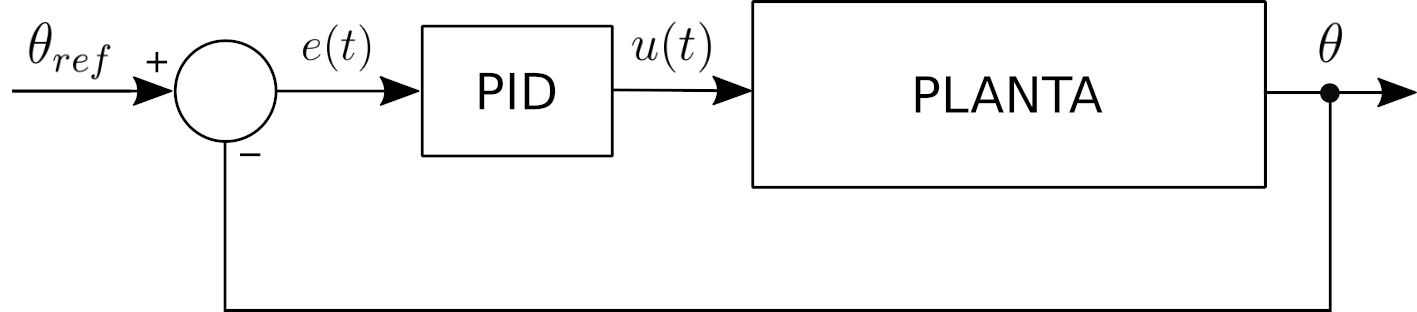
\includegraphics[width=0.5\textwidth]{background/PID_loop}
	\caption{Bucle de control realimentado con regulador PID}
	\label{PID_loop}
\end{figure}

La otra variante emplea un bucle de control en cascada, el cual consta de dos bucles cerrados de control. El bucle externo emplea un regulador P, este bucle genera la señal de referencia, para otro bucle de control interno, basado en la salida del sistema. El bucle interno emplea un regulador PID para controlar la magnitud de una variable interna. En el caso particular de este trabajo, el bucle externo intenta alcanzar una referencia de posición angular $\theta_{ref}$, para ello el regulador P, envía una referencia de velocidad angular $\dot \theta_{ref}$ a un controlador de velocidad con un regulador PID, vease \cref{PID_cascade_loop}.


\begin{figure}[htb!]
	\centering
	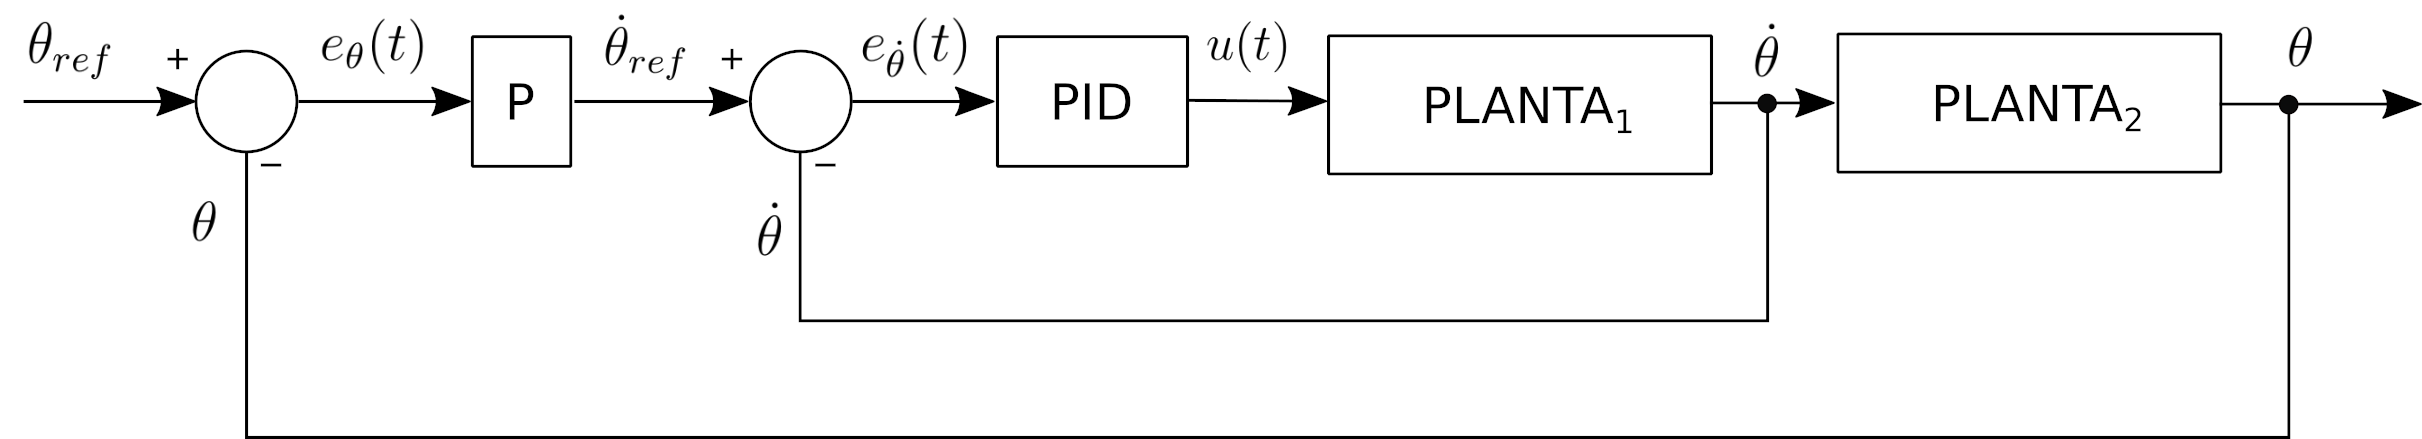
\includegraphics[width=0.9\textwidth]{background/PID_cascade_loop}
	\caption{Bucle de control en cascada}
	\label{PID_cascade_loop}
\end{figure}


\subsubsection{Control de la aeronave }
Para el control de la aeronave es necesario cerrar simultáneamente los 3 bucles de control, uno para cada ángulo. Cada bucle de control produce una salida $u_(t)$ a la planta, en este caso, a la aeronave. Para traducir estas señales a los comandos que se le envían a los motores, es necesario realizar una transformación. 


\begin{figure}[htb!]
	\centering
	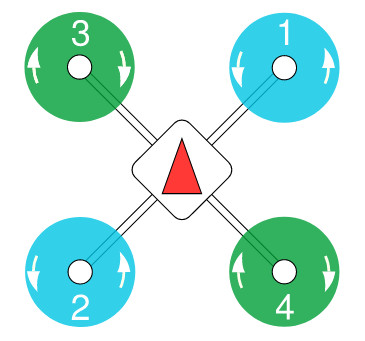
\includegraphics[width=0.3\textwidth]{introduccion/cuadrirrotorX.jpeg}
	\caption{Esquema cuadrirrotor en X}
	\label{Drone_en_X_Q}
\end{figure}


Intuitivamente, si se desea que el dron incline el morro hacia delante, la velocidad de los 2 motores traseros deberá aumentar, mientras que la velocidad de los motores delanteros deberá disminuirse. Si consideramos que inclinar el morro hacia delante implica que la nave tenga un ángulo $\theta > 0$ y que los motores estan dispuestos según la figura \ref{Drone_en_X_Q}, entonces 
\begin{align*}
	w_1 &= -\; u_\theta(t)\\
	w_2 &= +\; u_\theta(t)\\
	w_3 &= -\; u_\theta(t)\\
	w_4 &= +\; u_\theta(t)
\end{align*}

Si lo expresamos matricialmente:
\begin{equation}
	\left[\begin{array}{c}
		w_1\\
	w_2\\
	w_3\\
	w_4
	\end{array}\right] =\left[\begin{array}{c}
	-1 \\
	 +1 \\
	  -1 \\
	   +1
	\end{array}\right] u_\theta(t) 
\end{equation}

siendo $w_i$ la velocidad del motor i y $u_\theta(t)$ la salida del controlador de \textit{pitch}. Si se cierran los 3 bucles de control de forma simultánea y se suman las contribuciones de cada bucle sobre las acciones de control de forma similar


\begin{equation}
\left[\begin{array}{c}
w_1\\
w_2\\
w_3\\
w_4
\end{array}\right] =\underbrace{\left[\begin{array}{ccc}
-1 & -1 & +1 \\
+1 & +1 & +1 \\
-1 & +1 & -1 \\
+1 & -1 & -1
\end{array}\right]}_{\text{Matriz de transformación}}
\left[\begin{array}{c}
u_\varphi(t)\\
u_\theta(t)\\
u_\psi(t)
\end{array}\right]
\end{equation}

Esta matriz de transformación relaciona las salidas de los controladores con los comandos de los motores, modificando estos valores se puede aumentar la influencia de un bucle con respecto a otro.

\section{Redes neuronales artificiales} 
 Una red neuronal artificial (ANN) esta compuesta por un conjunto de nodos o perceptrones interconectados entre sí. Estos perceptrones se agrupan en capas ``ocultas'', se les atribuye este nombre debido a que todos los nodos de una capa se interconectan con todos los nodos de la capa anterior, por lo que después del aprendizaje de la red no se sabe cuales son los perceptrones de la capa anterior que influyen en un nodo.
 
 
 
 \begin{figure}[htb!]
 	\centering
 	\begin{tikzpicture}[]
 	\def\nodedist{35pt}
 	\def\layerdist{80pt}
 	\def\pindist{20pt}
 	
 	\tikzstyle{every pin edge}=[signal]
 	\tikzstyle{annot} = [text width=4em, text centered]
 	
 	\foreach \y in {1,...,3}
 	\node[inputnode, pin={[pin edge={latex-}, pin distance=\pindist]left:Entrada \y: $x_\y$}] 
 	(I\y) at (0,-\y*\nodedist) {$a_\y^{[0]}$};  
 	
 	\foreach \y in {1,...,4}
 	\node[hiddennode] 
 	(H\y) at ($(\layerdist,-\y*\nodedist) +(0, 0.5*\nodedist)$) {$a_\y^{[1]}$};
 	
 	\foreach \y in {1,...,1}
 	\node[outputnode, pin={[pin edge={-latex}, pin distance=\pindist]right:\Large$\hat y$}]
 	(O\y) at ($(I2) + (2*\layerdist, 0)$) {$a_\y^{[2]}$};
 	
 	\foreach \dest in {1,...,4}
 	\foreach \source in {1,...,3}
 	\draw[signal] (I\source) -- (H\dest);
 	
 	\foreach \dest in {1,...,1}
 	\foreach \source in {1,...,4}
 	\draw[signal] (H\source) edge (O\dest);
 	
 	\node[annot, above=4pt of H1] (hl) {Capa oculta};
 	\node[annot] at (I1 |- hl) {Capa de entrada};
 	\node[annot] at (O1 |- hl) {Capa de salida};
 	\end{tikzpicture}
 	\caption{Esquema de una red neuronal artificial}
 \end{figure}
 

Cada perceptron es la unidad mínima de computación de una ANN, estas unidades se dividen en dos partes, una parte lineal y una parte de activación o no lineal. En la parte lineal o parte ``Z'' se computa una regresión lineal de las salidas de los nodos anteriores.
 \begin{align}
 	z^{[l]}_i &= \sum_{j=0}^{n^{[l-1]}} {w_{ij}\cdot a^{[l-1]}_j} + b_i  \qquad &i=0,..,n^{[l]} \\
 	a^{[l]}_i &= g\left(z^{[l]}_i\right) \qquad  &i=0,..,n^{[l]}
 \end{align}
 El superíndice $[l]$ hace referencia a la capa en la que se encuentra el elemento. Siendo $n^{[l]}$ el número de nodos de la capa $l$-ésima.
 
 
 A los coeficientes $w_{ij}$ se les denomina los pesos del perceptrón y $b_i$ es el término independiente de la regresión. 
 
 
 \begin{figure}[htb!]
 	
 	\centering
 	\begin{tikzpicture}[
 	% define styles    
 	init/.style={ 
 		draw, 
 		circle, 
 		inner sep=2pt,
 		font=\Huge,
 		join = by -latex
 	},
 	squa/.style={ 
 		font=\Large,
 		join = by -latex
 	}
 	]
 	% Top chain x1 to w1
 	\begin{scope}[start chain=1]
 	\node[on chain=1] at (0,1.5cm)  (x1) {$a_1^{[l-1]}$};
 	\node[on chain=1,,label=above:\parbox{1cm}{pesos},join=by o-latex] (w1) {$w_1$};
 	\end{scope}
 	% Middle chain x2 to output
 	\begin{scope}[start chain=2]
 	\node[on chain=2] (x2) {$a_2^{[l-1]}$};
 	\node[on chain=2,join=by o-latex] {$w_2$};
 	\node[on chain=2,init] (sigma) {$\displaystyle\Sigma$};
 	\node[on chain=2,squa,label=above:{\parbox{2cm}{\centering Regresión lineal}}]   {$z_i^{[l]}$};
 	\node[on chain=2,squa,label=above:{\parbox{2cm}{\centering Función de\\ activacion}}]   {$a_i^{[l]}= g(z_i^{[l]})$};
 	\node[on chain=2,squa,label=above:Salida,join=by -latex] {$y_{out}$};
 	\end{scope}
 	% Bottom chain x3 to w3
 	\begin{scope}[start chain=3]
 	\node[on chain=3] at (0,-1.5cm) 
 	(x3) {$a_3^{[l-1]}$};
 	\node[on chain=3,join=by o-latex]
 	(w3) {$w_3$};
 	\end{scope}
 	% Bias
 	\node[label=above:\parbox{2cm}{\centering \text{$\;$} \\ $b$}] at (sigma|-w1) (b) {};
 	% Arrows joining w1, w3 and b to sigma
 	\draw[-latex] (w1) -- (sigma);
 	\draw[-latex] (w3) -- (sigma);
 	\draw[o-latex] (b) -- (sigma);
 	% left hand side brace
 	\draw[decorate,decoration={brace,mirror}] (x1.north west) -- node[left=10pt] {Entrada} (x3.south west);
 	
 	\end{tikzpicture}
 	\caption{Esquema de un perceptrón}
 	\label{esquema_perceptron}
 	
 \end{figure}
 
 La función $g(z)$ es la función de activación del nodo. Estas funciones proporcionan no linealidad a la red neuronal, permitiendo a estas la capacidad de generar modelos con grandes no linealidades. Las funciones de activación más frecuentes en la literatura son:
 
 \begin{itemize}
 	\item Función sigmoide: 
 	\begin{equation}
 	\sigma(z) = \frac{1}{1+e^{-z}} \qquad\qquad \sigma(z):\mathbb{R} \rightarrow [0,1]
 	\end{equation}
	\begin{figure}[htb!]
		\centering
		\begin{tikzpicture}[]
		\begin{axis}[ 
		%title=$\tanh(x)$,
		axis x line=middle, xmin=-4, xmax=4, xtick={-3,...,3}, xlabel=$x$,
		axis y line=middle, ymin=-2, ymax=2, ytick={-1,...,1}, ylabel=$f(x)$,
		legend pos=north west,
		legend style={empty legend, draw=none},
		scale only axis=true,
		width=8cm, height=4cm,
		thick,
		samples=101] 
		\addplot[blue, very thick] {1/(1+exp(-x))};
		%\addlegendentry{$\tanh(x)$}
		\end{axis}
		\end{tikzpicture}
		\caption{Función sigmoide}
	\end{figure}

	\item Tangente hiperbólica: 
	\begin{equation}
	\tanh(z) = \frac{e^z-e^{-z}}{e^z+e^{-z}} \qquad\qquad \tanh(z):\mathbb{R} \rightarrow [-1,1]
	\end{equation}
	
	\begin{figure}[htb!]
		\centering
		\begin{tikzpicture}[]
		\begin{axis}[ 
		%title=$\tanh(x)$,
		axis x line=middle, xmin=-4, xmax=4, xtick={-3,...,3}, xlabel=$x$,
		axis y line=middle, ymin=-2, ymax=2, ytick={-1,...,1}, ylabel=$f(x)$,
		legend pos=north west,
		legend style={empty legend, draw=none},
		scale only axis=true,
		width=8cm, height=4cm,
		thick,
		samples=101] 
		\addplot[blue, very thick] {tanh(x))};
		%\addlegendentry{$\tanh(x)$}
		\end{axis}
		\end{tikzpicture}
		
		\caption{Función tangente hiperbólica}
	\end{figure}

	\item ReLu (del inglés \textit{Rectified Linear Unit}): 
	
	\begin{equation}
		g(z) = \text{max}(0,z) \qquad\qquad g(z):\mathbb{R} \rightarrow [0,+\infty]
	\end{equation}
\\
	\begin{figure}[htb!]
		\centering
		\begin{tikzpicture}[]
		\begin{axis}[ 
		%title=$\tanh(x)$,
		axis x line=middle, xmin=-4, xmax=4, xtick={-3,...,3}, xlabel=$x$,
		axis y line=middle, ymin=-2, ymax=2, ytick={-1,...,1}, ylabel=$f(x)$,
		legend pos=north west,
		legend style={empty legend, draw=none},
		scale only axis=true,
		width=8cm, height=4cm,
		thick,
		samples=101] 
		\addplot[blue, very thick] {(\x < 0) * (0) + (\x > 0) * (\x)};
		%\addlegendentry{$\tanh(x)$}
		\end{axis}
		\end{tikzpicture}
		\caption{Función ReLu}
	\end{figure}
	

\end{itemize} 
  
 Para conseguir que la red neuronal realice predicciones precisas es necesario ajustar los pesos de la red, a este proceso es al que se denomina entrenamiento o aprendizaje. En el paradigma del aprendizaje supervisado este entrenamiento se realiza sometiendo a la red a ejemplos cuya salida es conocida. El objetivo de la red es minimizar el error de la esperanza de la estimación con respecto a la salida real del ejemplo. Formalmente, se define una función de coste $\mathcal{J}$ la cúal se quiere minimizar. Por ejemplo, una función de coste típica para problemas de clasificación binaria es la \textit{binary cross-entropy}:
 
 \begin{align}
 \mathcal{L}(\hat{y},y)&=-\big(y\log\hat{y} + (1-y)\log(1-\hat{y})\big)\\ 
 \mathcal{J}(w,b)&=\frac{1}{m}\sum_{i=1}^{m}{\mathcal{L}\big(\hat{y}^{(i)},{y}^{(i)}\big)}
 \end{align}
 donde $\hat{y}$ denota la estimación de la salida realizada por parte de la red, $y$ la salida conocida y $m$ el número de ejemplos. 
 
 Para minimizar esta función de coste, que depende de los pesos de la red, existen distintos métodos, uno de los más usados es el método del descenso de gradiente. Este método emplea la ``propagación hacia atrás'' (del inglés \textit{back propagation}) de la red neuronal, esto consiste en obtener las derivadas parciales de la función de coste con respecto a los pesos de cada nodo y actualizar estos pesos en la dirección opuesta al máximo gradiente.
 
 \begin{align}
 	w:= w - \alpha\; &\frac{\partial\mathcal{J}(w,b)}{\partial w}\\
 	b:= b - \alpha\; &\frac{\partial\mathcal{J}(w,b)}{\partial b}
 \end{align}
 
 donde $\alpha$ denota la tasa de aprendizaje, es decir, lo rápido que varian estos pesos.

 



\section{Aprendizaje por refuerzo}

El aprendizaje por refuerzo o \textit{Reinforcement learning} \cite{sutton2018reinforcement} es un área del aprendizaje automático o \textit{Machine Learning} en el que un agente interactúa con un entorno buscando la mejor acción a realizar en función de su estado actual, de manera que maximice las recompensas acumuladas en el tiempo.


\begin{figure}[htb!]
	\centering
	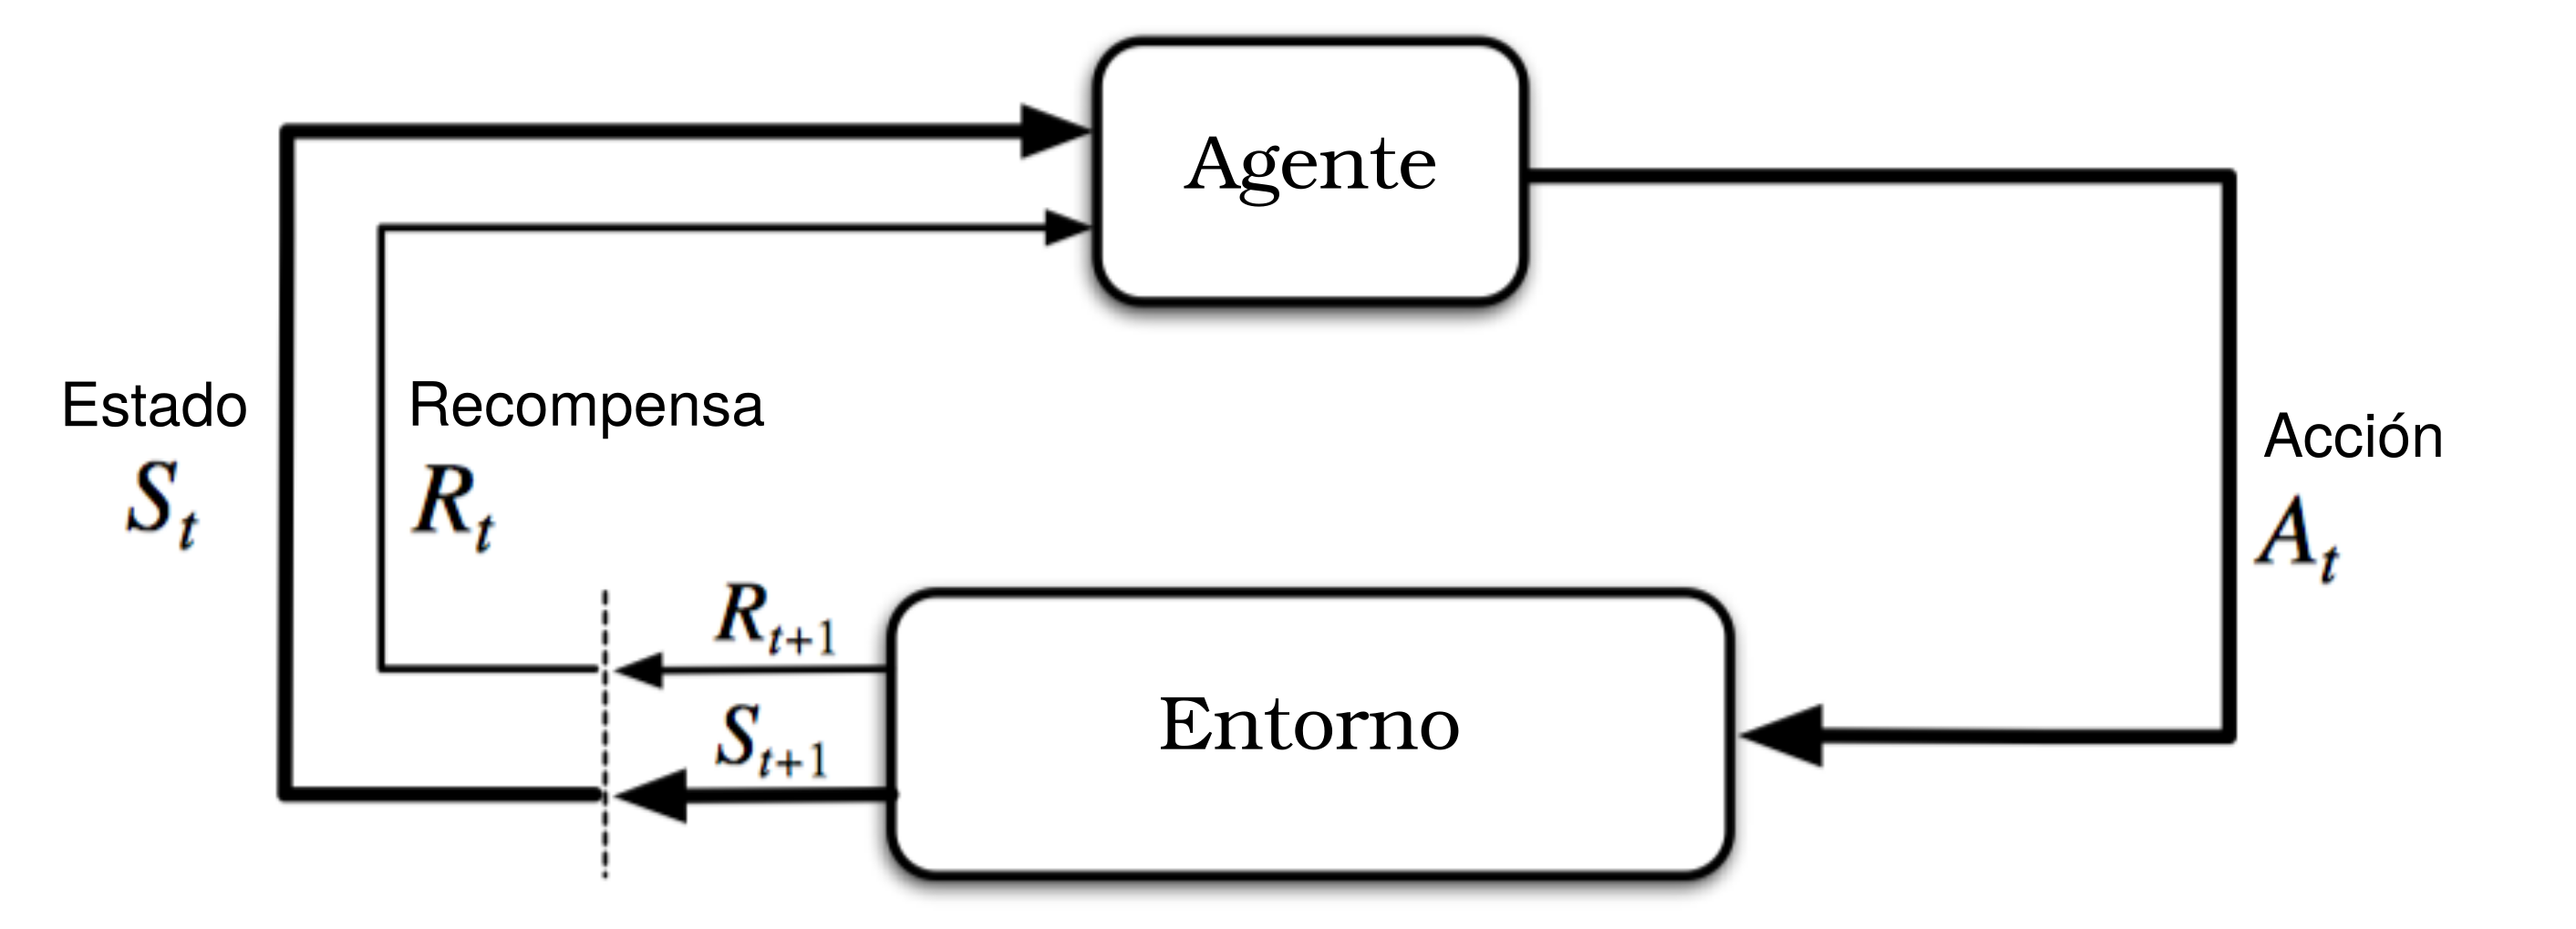
\includegraphics[width=0.8\textwidth]{background/RL_diagram}
	\caption{Diagrama canónico del bucle de interacción entorno-agente}
	\label{Rl-diagram}
\end{figure}


Se diferencia de otras técnicas de aprendizaje automático es su enfoque orientado a la interacción directa con el entorno, sin basarse en un modelo completo del entorno o en un conjunto de ejemplos supervisados.

\subsubsection{Elementos del aprendizaje por refuerzo}
Además del agente y el entorno se pueden identificar tres elementos principales más en un sistema de aprendizaje con refuerzo:

\begin{itemize}
	\item[$\bullet$] \textbf{Política ($\pi$)}  (Proveniente del termino anglosajón \textit{policy}, el cual es el término empleado en el estado del arte). Define el conjunto de acciones que debe realizar el agente para conseguir maximizar su recompensa en función su estado, el cuál es percibido a través del entorno. La \textit{policy} constituye el núcleo del agente y nos permite determinar su comportamiento. Estas políticas pueden ser estocásticas.
	
	\item[$\bullet$] \textbf{Recompensa} ($R_t$). 
	Define el objetivo del agente en un problema de aprendizaje por refuerzo. En cada salto de tiempo (\textit{step}) el agente recibe una recompensa por parte del entorno. 
	
	\item[$\bullet$] \textbf{Función de valor} ($V^\pi_s$). Representa la máxima recompensa que puede esperar obtener un agente desde un estado concreto, empleando una política concreta, es decir, tiene en cuenta la recompensa a largo plazo, no solo la inmediata.
	\begin{equation}
		V^\pi(s)= \mathbb{E}_\pi\left[\sum_{k=0}^{\infty}{\gamma^k r_{t+k+1}}\Big|s_t=s\right]
	\end{equation}
		
\end{itemize}
Algunos algoritmos de aprendizaje por refuerzo requieren de la definición de un \textbf{modelo del entorno}. Este modelo permite predecir el comportamiento que va a tener el entorno a lo largo del tiempo. Los algoritmos que emplean un modelo se les denomina \textit{model-based}, mientras que, a los algoritmos que no requieren de un modelo del entorno se les denomina \textit{model-free}.

\subsubsection{Procesos de decisión de Markov}

El aprendizaje por refuerzo emplea el marco formal de los procesos de decisión de Markov (\textit{MDP}) en los cuales para definir la interacción entre en agente y el entorno en términos de estados, acciones y recompensas.

Un proceso de decisión de Markov está compuesto por la 4-tupla $(S,A,P_a,R_a)$ donde:

\begin{itemize}
	\item \textbf{S} representa el estado del agente.
	\item \textbf{A} es el conjunto de acciones que puede realizar el agente. $A_s$ denota las acciones que puede realizar el agente desde un estado $s$.
	\item \textbf{$\boldsymbol{P_a(s,s')}$} = $Pr\big(s_{t+1} = s' \;|\; s_t = s , a_t = a  \big)$. Partiendo de un estado $s$, $P_a$ representa la probabilidad de pasar al estado $s'$ tomando la acción $a$.
	\item \textbf{$\boldsymbol{R_a(s,s')}$} denota la recompensa inmediata que recibiría el agente al realizar la transicion de $s$ a $s'$ mediante la acción $a$.
\end{itemize}

Estos procesos cumplen la propiedad de Markov, es decir, que el pasado no influye en el agente, lo único relevante es el estado actual.

El problema principal de los MDP es encontrar la secuencia de acciones que debe realizar el agente para maximizar la recompensa a largo plazo, es decir, encontrar la política $\pi$ 
óptima, que permita maximizar la recompensa. Una vez encontrada la política $\pi$ óptima el problema se reduce a una cadena de Markov, dado que la acción $a$ a realizar en un estado $s$ viene completamente definida por el estado $s$ y la probabilidad $P_a$. 

La política $\pi$ óptima es aquella que maximice la recompensa acumulada, es decir, la suma descontada de las recompensas instantáneas percibidas por el entorno:

\begin{equation}
	G_t = R_{t+1} + \gamma R_{t+2} + \gamma^2 R_{t+3} + ... = \sum_{k=0}^{\infty}\gamma^k R_{
	t+k+1}
\end{equation}

donde $\gamma$ es el factor de descuento, el cual debe cumplir $0 \le \gamma \le 1$, cuanto mayor sea este factor menos importante es la recompensa inmediata. 


\subsection{Algoritmos de \textit{Q-learning}}
En este trabajo se han trabajado con 2 tipos de algoritmos de aprendizaje por refuerzo: métodos basados en \textit{Q-learning} y métodos de gradiente de las políticas.


Los algoritmos de Q-learning se basan en la función estado-acción, también conocida como función Q, de ahí el nombre de estos algoritmos. Esta función denota el valor de tomar una acción para un estado concreto, siguiendo una política $\pi$. Formalmente, la función Q se define como

\begin{equation}
	Q^\pi(s,a) =  \mathbb{E}_\pi\left[\sum_{k=0}^{\infty}{\gamma^k r_{t+k+1}}\Big|s_t=s,a_t = a\right]
\end{equation}

La diferencia entre la función Q y la función de valor radica en que la función de valor cuantifica el valor, en términos de recompensa acumulada, que posee un estado concreto, mientras que la función Q evalúa la conveniencia de tomar una acción concreta en un estado determinado. Este matiz se empleará posteriormente para definir la función de ventaja en el apartado \ref{ALG_GRAD_POL}.

El objetivo de estos algoritmos se basa en obtener la función óptima $Q^*$, esta función cumple la ecuación de Bellman 
	\begin{equation}
		Q^*(s,a)= \mathbb{E}_{s'}\left[r+\gamma\;\underset{a'}{\text{max}}\; Q^*(s',a')\big|s,a\right]
	\end{equation}
siendo s'y a' la secuencia siguiente de estados y acciones, respectivamente.

Basándose en esta ecuación la función $Q^*$ se podría calcular como un proceso iterativo de la forma
	\begin{equation}
	Q_{i+1}(s,a)= \mathbb{E}\left[r+\gamma\;\underset{a'}{\text{max}}\; Q_i(s',a')\big|s,a\right]
	\end{equation}

Aunque este proceso converge a la funcion estado-acción óptima, $Q_i \rightarrow Q^*$ cuando $i \rightarrow \infty$ \cite{sutton2018reinforcement}, esto no es práctico, debido a que esta aproximación de la función Q se estima de forma independiente para cada secuencia concreta, sin generalizar. En lugar de esto, se suele emplear una función que se aproxime a esta función estado-acción. En los casos en los que esta función sea aproximada por una red neuronal, ésta se denota por $Q(s,a; \theta)$ siendo $\theta$ los pesos de esta red-Q (\textit{Q-network}). 

La función de pérdida que se intenta minimizar para entrenar esta red es
\begin{equation}\label{eq:1}
	L_i(\theta_i) = \mathbb{E}_{s,a\sim\rho(s,a)}\left[\left(y_i - Q(s,a;\theta_i)\right)^2\right]
\end{equation} 
donde $y_i= \mathbb{E}_{s'}[ r + \gamma \; {\text{max}_{a'}} \; Q(s',a';\theta_{i-1})]$ es el objetivo(\textit{target}) para la iteración i y $\rho(s,a)$ es la distribución del comportamiento, es decir, distribución de probabilidad de las secuencias $a', s'$ a lo largo del tiempo.

Esta función de pérdida se puede minimizar con algoritmos de optimización como el Descenso de gradientes estocástico (SDG).

\subsubsection{DQN}

El algoritmo DQN (\textit{Deep Q-network}) es un algoritmo basado en \textit{Q-learning} desarrollado por Mnih et al. \tb{citar} en 2015. Con este algoritmo la empresa DeepMind consiguió desarrollar un agente capaz de jugar a los juegos de la clásica consola Atari, superando con creces el rendimiento de los jugadores profesionales en algunos juegos. Este algoritmo está diseñado para actuar sobre un conjunto de acciones discretas, como son las acciones de la consola Atari.

El nombre del algoritmo, hace referencia al empleo de una red neuronal profunda (\textit{Deep Network}) como aproximador de la función Q (\textit{Q-network}).
Este algoritmo introduce, principalmente, dos modificaciones sobre los algoritmos Q que favorecen el aprendizaje:

\begin{enumerate}
	\item \textbf{Creación de un ``contenedor de repeticiones''} (\textit{buffer replay}) en el que se almacenan las experiencias del agente en cada iteración temporal $e_t=(s_t,a_t,r_t,s_{t+1})$ en un conjunto de datos $D_t=\{e_1,...,e_t\}$ recabados durante varios episodios.
	
	Este contenedor se emplea para obtener una muestra de aleatoria de experiencias y constituir un pequeño lote con el que optimizar la red-Q.
	
	Emplear este método proporciona proporciona varias ventajas notorias:
	
	\begin{itemize}
		\item Permite el empleo de los datos recabados en cada paso temporal para optimizar los pesos en múltiples interacciones, lo que se traduce en un mejor aprovechamiento de las experiencias del agente.
		
		\item Al tomar muestras de forma consecutiva el aprendizaje se vuelve ineficiente debido a la alta correlación entre las muestras. Al tomar muestras aleatorias del contenedor se consigue romper esta correlación.
	\end{itemize}
	
	\item \textbf{Empleo de una red objetivo }$Q'$ para la actualización de pesos.  Cada $C$ actualizaciones se clona la red $Q$ para obtener la red objetivo $\hat Q$. Esta red objetivo $\hat Q$ es la que emplea para realizar el cómputo de la expresión $y_i$ durante la actualización de pesos.
	\begin{equation}
	y_i= \mathbb{E}_{s'}[ r + \gamma \; {\text{max}_{a'}} \; \hat Q(s',a';\theta^-)]
	\end{equation}
	En este algoritmo se realiza la optimización mediante el algoritmo SDG de la funcion de pérdida \ref{eq:1}.  Cada $C$ pasos se reinicia la función Q con los valores del objetivo $Q=\hat Q$.
	
	Al emplear una red con parámetros desactualizados, a la hora de actualizar la red, se  reduce las oscilaciones en el entrenamiento y se favorece la convergencia.
	
\end{enumerate}

En este algoritmo, la política $\pi$ que dicta que acción $a$ es la más conveniente en un estado $s$ determinado se obtiene a partir de la función Q de forma inmediata

\begin{equation}		
		a_t(s) = \text{argmax}_a\;Q(s,a|\theta) 
\end{equation}

es decir, se escoge la acción $a$ que maximice la función Q en ese estado.
\subsubsection{DDPG}

El algoritmo DDPG (\textit{Deep Deterministic Policy Gradient}), creado por Lillicrap et al. \tb{citar} en 2016, adapta las ideas del DQN a un dominio de acciones continuo. Este algoritmo emplea la filosofía \textit{actor-critic}, en la que una parte evalúa el valor de una accion en un estado (crítico) y  otra define la política que debe realizar el agente (actor).

La función actor $\mu(s|\theta^\mu)$ devuelve la acción que se debe realizar en el estado $s$, es decir, la política $\pi$ que debe seguir el agente. El crítico $Q(s,a)$ se entrena empleando la identidad de Bellman al igual que en los algoritmos de \textit{Q-learning}.

Para actualizar los pesos de la función actor se emplea el gradiente de la función de coste empleados por Silver et al. \tb{citar DPG paper} 

	\begin{align}
		\nabla_{\theta^\mu}J &\approx \mathbb{E}_{s_t \sim \rho}\left[ \nabla_{\theta^\mu} Q(s,a |\theta^Q)|_{s=s_t,a=\mu(s_t|\theta^\mu)}\right]\\
		&=  \mathbb{E}_{s_t \sim \rho}\left[ \nabla_{a} Q(s,a |\theta^Q)|_{s=s_t,a=\mu(s_t)} \nabla_{\theta^\mu}\; \mu(s|\theta^\mu)|_{s=s_t}    \right]\nonumber 
	\end{align}

Para favorecer la exploración del algoritmo se genera una política de exploración $\mu'$ se le añade ruido $\mathcal{N}$ a la política del actor
	\begin{equation}
		 \mu'(s_t)=\mu(s_t|\theta^\mu_t) + \mathcal{N}
	\end{equation}

este ruido se puede generar de varias formas, en el artículo se emplea ruido generado mediante el proceso de Ornstein-Uhlenbeck \tb{(citar)} para generar ruido correlado temporalmente.

Este algoritmo mantiene el contenedor de repeticiones y el empleo de redes objetivo del DQN aunque añade alguna modificación en esta última. En vez de reiniciar el valor de la red  con el valor de la red objetivo cada $C$ épocas, en el DDPG, esta actualización de las redes $Q$ y $\mu$ se realiza de forma suave mediante una media ponderada móvil.
\begin{align}
\theta ^{\hat Q} &\leftarrow \tau \theta ^ Q + (1 - \tau)\theta^{\hat Q}\\
\theta ^{\hat \mu} &\leftarrow \tau \theta ^ \mu + (1 - \tau)\theta^{\hat \mu}
\end{align}
con $\tau \ll  1$. De esta forma los pesos de la red cambian de forma suave, lo que favorece la estabilidad del entrenamiento. 

\subsection{Algoritmos de gradiente de política} \label{ALG_GRAD_POL}

En los algoritmos de \textit{Q-learning} es objetivo es encontrar una función $Q(s,a|\theta)$ que se aproxime lo máximo a la función $Q^*$, para a partir de esta función extraer la política óptima.
En cambio, en los algoritmos de gradiente de política (\textit{policy gradients}) lo que se parametriza, es una política $\pi_\theta$, por lo que el objetivo  de estos algoritmos es encontrar los parámetros que maximizan la recompensa acumulada . La función de coste a maximizar de estos algoritmos es directamente

\begin{equation}
J(\theta)=\mathbb{E}_\pi[r(\tau)]	
\end{equation}
siendo $r(\tau)$ la recompensa total obtenida al realizar una trayectoria $\tau$. Si se emplea un algoritmo de optimización basado en el descenso de gradientes los pesos se actualizarían de la siguiente forma
\begin{equation}
	\theta_{t+1} = \theta_t + \alpha \nabla J (\theta_t)
\end{equation}
por lo que el objetivo es encontrar el gradiente $\nabla J (\theta_t)$ e iterar en el tiempo para obtener la política optima. El teorema del gradiente de política \tb{citar} se obtiene que 

\begin{equation}\label{eq:2}
	\nabla J (\theta_t) = \mathbb{E}_\pi\left[\sum_{t=0}^{\infty}\gamma^t  \nabla_\theta \log \pi_\theta(a_t|s_t) A^{\pi_\theta}(s_t,a_t)\right]
\end{equation} 

	Siendo $A^\pi$ la función de ventaja, definida como 
	\begin{equation}
	A^\pi(s_t,a_t)=Q^\pi(s_t,a_t) - V^\pi(s_t)
	\end{equation}
intuitivamente, la función de ventaja representa el beneficio o perjuicio de elegir la acción $a_t$ en lugar de seguir la política $\pi$ en un estado determinado. Al emplear esta función en la expresión \ref{eq:2} la política evoluciona hacia las acciones que consiguen una recompensa mayor que la acción media.

\subsubsection{TRPO}

El algoritmo TRPO \textit{(Trust Region Policy Optimization)} es un algortimo desarrollado por Schulman et al. \tb{citar} en 2017, que emplea el concepto de la región de confianza (\textit{Trust Region}) para favorecer la convergencia del entrenamiento.

La región de confianza limita el cambio que puede sufrir la política en cada iteración, de esta forma, primero se establece el tamaño máximo del paso y posteriormente se localiza el punto óptimo dentro de esta región.

En este algoritmo se intenta
\begin{align}\label{eq:3}
	\underset{\theta}{\text{Maximizar}}\qquad&{\mathbb{\hat E}_t} \left[ \frac{\pi_\theta (a_t|s_t)}{\pi_{\theta_{old}} (a_t|s_t)} \hat{A}_t\right]\\\label{eq:4}
	\text{Sujeto a}\qquad& {\mathbb{\hat E}_t} \left[ \text{KL}[\pi_{\theta_{old}}(\cdot|s_t),\pi_{\theta}(\cdot|s_t)]\right] \le \delta
\end{align}

La expresión \ref{eq:3} es una función límite inferior a $J(\theta^*)$, es decir, para cualquier valor de $\theta \neq \theta^*$, todos los puntos de la expresión \ref{eq:3} se encuentran por debajo de la función $J(\theta^*)$. Esto implica que se pueden emplear métodos de minorización-maximización (algoritmos MM), los cuales van aproximando una función limite inferior, a otra, límite superior mediante iteraciones (\cref{MM_fig}).

\begin{figure}[htb!]
	\centering
	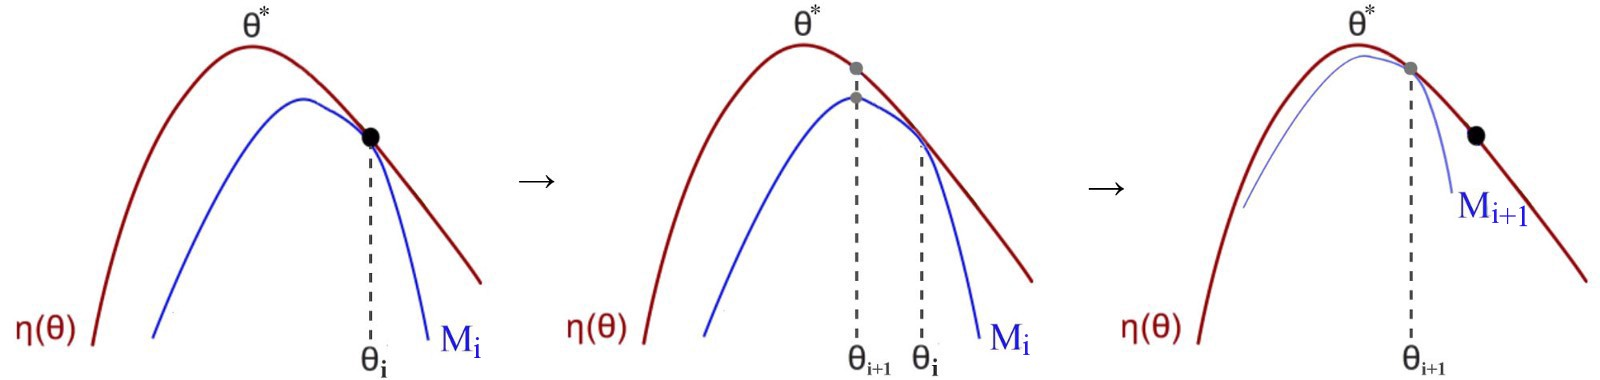
\includegraphics[width=0.9\textwidth]{background/MM}
	\caption{Evolución de una función limite inferior con un algoritmo MM.}
	\label{MM_fig}
\end{figure}

Al emplear este método, junto con las limitaciones impuestas con la región de confianza, se consigue mejorar la convergencia del entrenamiento a la solución óptima.

\subsubsection{PPO}
El algoritmo PPO (\textit{Proximal Policy Optimization}), fue desarrollado por Schulman et al. \tb{cite} en 2017, como una mejora del algoritmo TRPO explicado anteriormente. El algoritmo TRPO tiene una complejidad de implementación muy elevada, el objetivo PPO era simplifica esta complejidad y consigue mejorar el rendimiento de su predecesor.

Este algoritmo tiene dos variantes, aunque, en este trabajo, solamente se tratará sobre la variante que ``recorta'' el objetivo (\textit{Clipped Surrogate Objetive}).

Sea $r_t(\theta)$ el radio de probabilidad $r_t(\theta) = \frac{\pi_{\theta}(a_t|s_t)}{\pi_{\theta_{old}(a_t|s_t)}}$, empleando esto en la expresión de la función objetivo del TRPO (eq. \ref{eq:3})

\begin{equation}
	L^{\text{CPI}}	(\theta)={\mathbb{\hat E}_t} \left[ \frac{\pi_\theta (a_t|s_t)}{\pi_{\theta_{old}} (a_t|s_t)} \hat{A}_t\right]
	= 	{\mathbb{\hat E}_t} \left[ r_t(\theta)\hat{A}_t\right]
\end{equation}

Si no hubiera ninguna limitación, al maximizar $L^{\text{CPI}}$, se realizarían cambios muy grandes de la política. Es por esto que Schulman et al. se plantean como modificar esta función para penalizar cambios grandes en las políticas, los cuales distancian $r_t(\theta)$ de 1. La función objetivo que proponen

\begin{equation}
	L^{\text{CLIP}}	(\theta) = 	{\mathbb{\hat E}_t} \left[ \text{min} \left(r_t(\theta)\hat{A}_t \;,\; \text{clip}(r_t(\theta),1-\epsilon,1+\epsilon )\;\hat{A}_t \right) \right]
\end{equation}

donde $\epsilon$ es un hiperparámetro, por ejemplo, $\epsilon = 0.2$. De esta forma, se limita que se potencien mucho las acciones realizadas, cuando la ventaja es positiva y que , cuando la ventaja sea negativa, no se rechacen de forma permantente las acciones realizadas, véase \cref{ppo_clip}.
\begin{figure}[htb!]
	\centering
	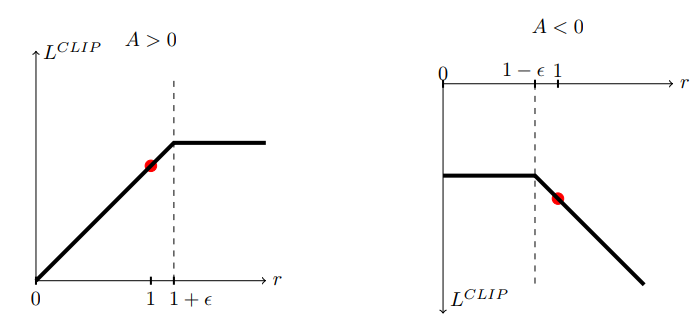
\includegraphics[width=0.9\textwidth]{background/ppo_clip}
	\caption{Gráficas de la función objetivo $L^{\text{CLIP}}(\theta)$ para distintos valores de $r$, dependiendo del signo de la ventaja $A$}
	\label{ppo_clip}
\end{figure}

De esta manera, la función objetivo se puede optimizar con un un optimizador de primer order, por lo que, aunque a veces se tomen algunas acciones erroneas, se consigue obtener un mejor rendimiento de una forma mucho mas sencilla al TRPO.

	\chapter{Hardware}

Con el ánimo de tener una plataforma real sobre la que probar el rendimiento de los algoritmos de control diseñados, se ha diseñado y construido un cuadrirrotor \textit{ad hoc} para este propósito.

Un cuadricóptero convencional cuenta con: un chasis o cuadro que lo sustenta, cuatro motores y la electrónica necesaria para controlarlos, una controladora de vuelo que lo comanda y baterías que le proporcionan energía.

A continuación se detallará como son las distintas partes físicas del dron que se ha fabricado.

\section{Cuadro}
El \textit{frame} está compuesto por perfiles de aluminio y piezas de PLA fabricadas mediante impresión 3D de diseño propio. La estructura básica está formada por 5 conjuntos de piezas distintos:
\begin{itemize}
	\item[$\bullet$] \textbf{Portamotores}: son las piezas donde se alojan los motores. Para conseguir una buena fijacion los motores se atornillan a los portamotores empleando 4 tornillos dispuestos seǵun los vértices de un rombo.
	
	\tb{Imagen}
	
	\item [$\bullet$] \textbf{Brazos}: se encargan de unir los portamotores con el \textit{núcleo} de la estructura. En este diseño, los brazos consisten en perfiles de aluminio de sección cuadrada de 8mm de lado.
	
	\item [$\bullet$] \textbf{Núcleo}: Es la pieza principal del diseño, en la que se anclan el resto de las partes y donde se alojan los componentes electrónicos. Esta pieza sustenta los brazos y el porta-baterias de la aeronave. Cuenta con agujeros a medida para poder situar el autopiloto y los variadores.
	
	\tb{Imagen}
	 
	\item [$\bullet$] \textbf{Separadores}: su propósito es mantener unidos el \textit{núcleo} y el porta-baterías manteniendo una separación fija entre ellas.
	
	\tb{Imagen}
	
	\item [$\bullet$] \textbf{Porta-baterías}: Es la parte inferior del cuadricóptero. En ella se apoya la batería Li-Po que alimenta al dron y se mantiene anclada durante el vuelo. Además posee unas protuberancias cuya función se asemejaría a las de un tren de aterrizaje.  
	
	\tb{Imagen}
	
	  
\end{itemize} 

\section{Motores y hélices}
El dron cuenta con 4 motores sin escobillas (\textit{brushless}) LHI MT2204 II de 2300KV con una tensión de alimentación entre 7.2 V y 11.1 V (2s -3s en una batería LiPo) y una corriente continua máxima de 16A.

\begin{figure}[htb!]
	\centering
	\begin{subfigure}{0.4\textwidth}
		\centering
		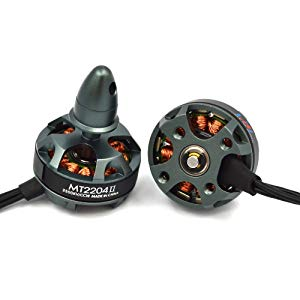
\includegraphics[height=0.2\textheight]{hardware/motores.jpg}
	\end{subfigure}
	\begin{subfigure}{0.4\textwidth}
	\centering
	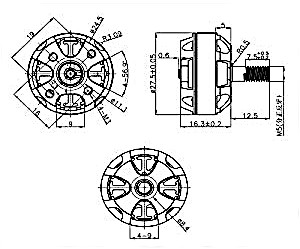
\includegraphics[height=0.2\textheight]{hardware/motoresPlanos}
\end{subfigure}
	\caption{Motores LHI MT2204 II empleados}
\label{hardware:motores}
\end{figure}

Se ha estimado que el peso aproximado de la aeronave se encuentra entorno a los 800 gramos. La literatura recomienda que los motores que se escojan deben tener empuje suficiente para poder levantar el doble del peso de la aeronave. Observando la tabla de especificaciones de los motores, se observa que, la hélice HQ5040 proporciona empuje suficiente con un ratio empuje/potencia bastante elevado, como se puede observar en la \cref{hardware:motoresTabla}.

\begin{figure}[htb!]
	\centering
	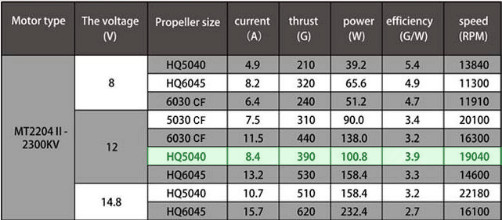
\includegraphics[width=0.7\textwidth]{hardware/MT2203_Table.jpeg}
	\caption{Tabla de especificaciones motor MT2204 II. }
	\label{hardware:motoresTabla}
\end{figure}

Es por esto que se han empleado hélices tripala HQ5040 de policarbonato y fibra de vidrio (\cref{hardware:helice}).

\begin{figure}[htb!]
	\centering
	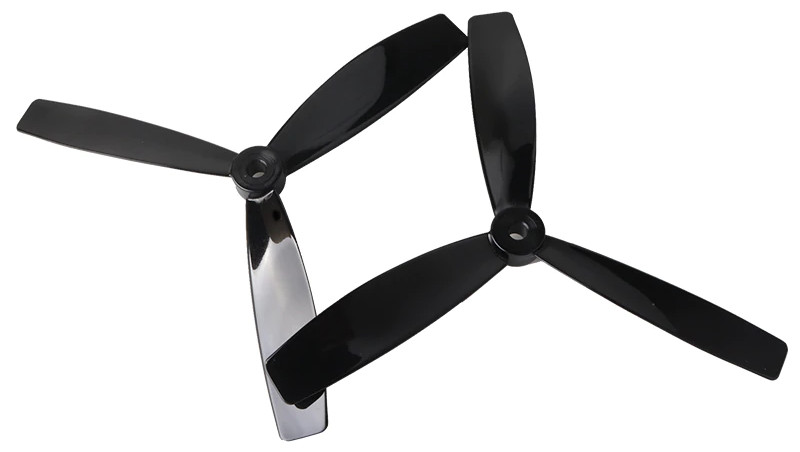
\includegraphics[width=0.5\textwidth]{hardware/helices.jpeg}
	\caption{Hélices tripala HQ5040}
	\label{hardware:helice}
\end{figure}

\section{Variadores (ESC)}


Los motores  que se han escogido son trifásicos, es decir, se alimentan con 3 corrientes alternas monofásicas de igual frecuencia y amplitud, desfasadas 120\grad \;eléctricos. Para obtener estás formas de ondas a partir de la corriente continua de las baterias, se utilizan los variadores.

Un variador o \textit{ESC (Electronic Speed Control)} es un circuito electrónico que se encarga de generar las ondas eléctricas necesarias para controlar y regular la velocidad de un motor eléctrico. Cuenta con un microcontrolador, el cual se encarga de conmutar los interruptores de potencia, con el ánimo de alimentar las distintas fases del motor de forma sincronizada, haciendo que gire a la velocidad deseada, veáse la \cref{hardware:esc_explicacion}.
\begin{figure}[htb!]
	\centering
	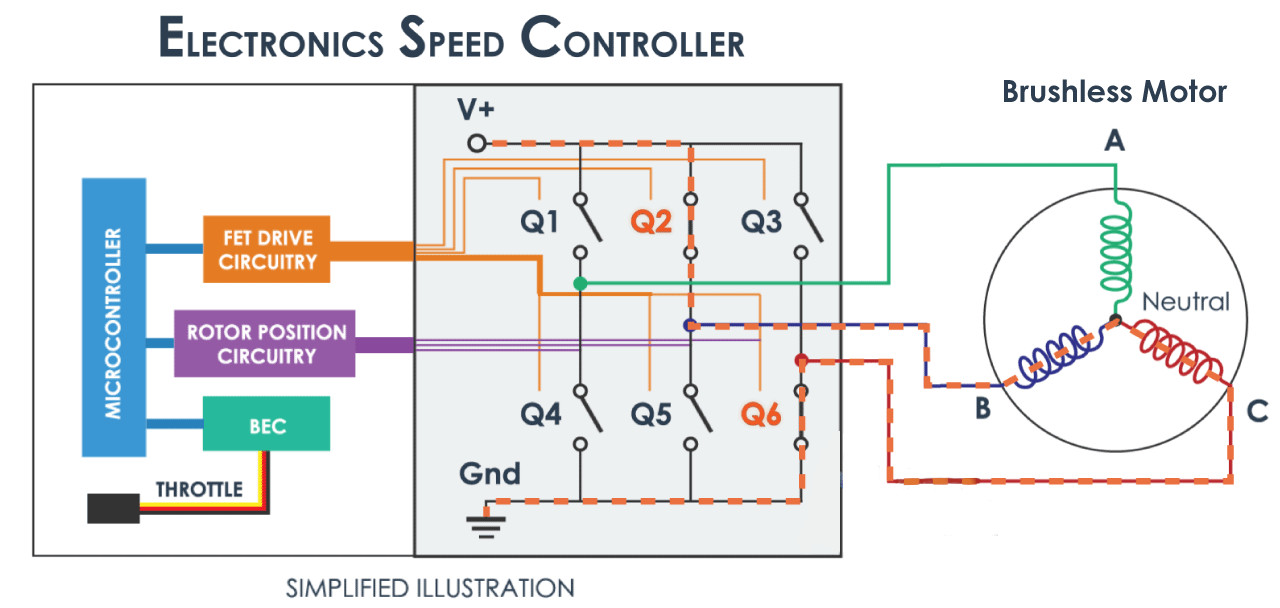
\includegraphics[width=0.6\textheight]{hardware/howtomecatronics}
	\caption{Funcionamiento ESC (www.howtomechatronics.com)}
	\label{hardware:esc_explicacion}
\end{figure}

Para el cuadricóptero se ha optado por emplear un variador BLHeli Multistar Race (\cref{hardware:esc}) que integra 4 variadores en uno, es decir se pueden alimentar 4 motores trifasicos con él. Estos variadores soportan una corriente de hasta 30 A cada uno.

\begin{figure}[htb!]
	\centering
	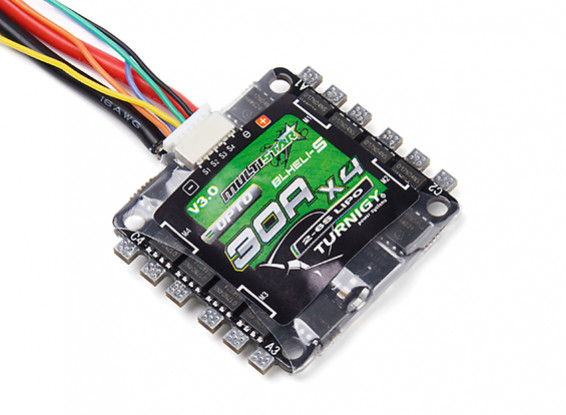
\includegraphics[height=0.2\textheight]{hardware/esc.jpg}
	\caption{ESC Multistar Race 4 in 1 30A BLHeli empleado}
	\label{hardware:esc}
\end{figure}

\section{Baterias}
Para alimentar al dron, se han elegido baterias tipo LiPo por su alta tasa de descarga (la batería que se ha escogido es capaz de entregar hasta 130 A) y la su estabilidad en la tensión mientras están cargadas.


\begin{figure}[htb!]
		\centering
		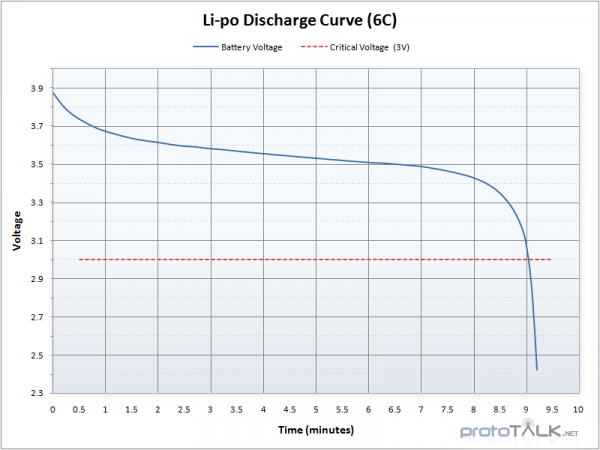
\includegraphics[width=0.8\textwidth]{hardware/curvaLipo}
		\caption{Curva típica de descarga de una bateria LiPo (fuente: ProtoTalk.net)}
		\label{hardware:curvaLipo}

\end{figure}


\section{Autopiloto}

En los drones, el sistema que se encarga de estabilizar al cuadricóptero y hacerlo pilotable se denomina la controladora de vuelo o el Autopiloto. Existe una gran variedad de controladoras en el mercado, pero para este trabajo se ha diseñado una controladora propia con el fin de poder tener acceso a todos los sensores y a implementar el algoritmo de control de forma óptima. El autopiloto consta de 3 partes diferenciadas: la electrónica de potencia, el microcontrolador y los sensores. A continuación \tb{se tratará} sobre estas partes con más detalle.\\


\tb{Estaría bien un par de imágenes de la PCB (anverso y reverso)}\\

\begin{figure}[htb!]
	\centering
	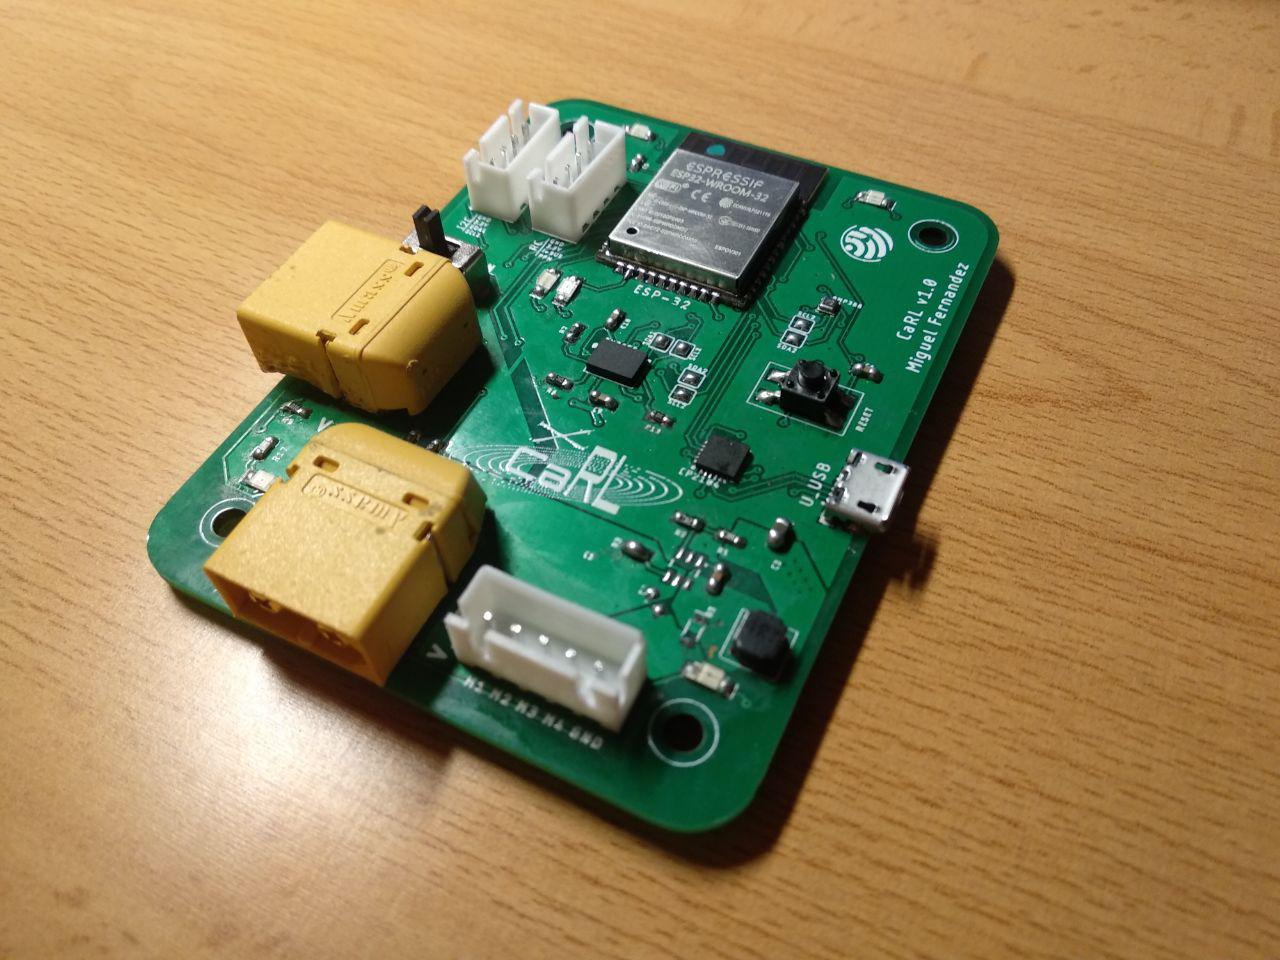
\includegraphics[width=0.8\textwidth]{hardware/carl_board}
	\caption{Autopiloto CaRL (\textit{Cuadcopter with autopilot based on Reinforcement Learning}).}
	\label{hardware:carl_board}	
\end{figure}



\subsection{Fase de Potencia}

Con el fin de poder gestionar la potencia entregada por las baterias a la placa y a los motores se ha diseñado una etapa de potencia en la que se debe mencionar dos partes: el interruptor de potencia y el regulador a 3.3 Voltios.

\subsubsection{Interruptor de potencia}

Los motores del dron pueden llegar a consumir 12 Amperios cada uno, lo que los cuatro motores pueden llegar a consumir 48 Amperios. Un interruptor con tamaño reducido no puede manejar tanta corriente, por ello se ha empleado un transistor MOSFET de canal P por el que pueden circular hasta 100 Amperios, con el fin de abrir o cerrar el paso de corriente desde las baterías al resto de la placa. El MOSFET se controla con un interruptor de poca potencia entre drenador y puerta.\\

Cuando se cierra el interruptor se alimenta directamente al ESC y al regulador de tensión.


\subsubsection{Regulador a 3.3V}

La eléctronica digital de la PCB se alimenta y emplea lógica a 3.3 Voltios, por lo que no la podemos conectar a las baterías de 11.1 Voltios.  Para adecuar la tensión se ha escogido un regulador Step-down de tipo Buck (Figura \ref{hardware:Buck}) \tb{(¿explico como funciona un convertidor Buck?)}. El circuito integrado que se encarga de conmutar la fuente es el chip AP3211.
\begin{figure}[htb!]
	\centering
		\begin{circuitikz}[american voltages,european resistors,scale=1]	
		
		\draw
		(0,2) to [V=$V_{in}$]  (0,-2)
		(0,2) to ++(1.5,0)
		++(0.5,0)node[nigfete,bodydiode,rotate=90]{}  to ++(2,0);
		
		\draw 
		(0,-2) to ++(4,0)
		++(0,0)[sD*] to ++(0,4)
		;
		\draw 
		(4,2) to [L=$L$,i=$i_L$] ++(3,0);
		\draw
		(7,2) to [C,l_=$C$] ++(0,-4)
		;
		
		\draw
		(7,2) to ++(3,0) 
		to [R =$R_{load}$,i=$i_{Load}$] ++(0,-4)
		to (0,-2)
		;
		\draw (2,0.75)node[]{\footnotesize SW};
		\draw (9.5,0.5)[short] to ++ (0,-0.5);
		\draw[-latex]
		(9.5,0)node[left] {$V_{out}$} to ++(0,-0.5);	
		
	\end{circuitikz}
	\caption{Esquema de un convertidor Buck}
	\label{hardware:Buck}
\end{figure}


\subsection{El microcontrolador (ESP32)}

El microcontrolador por el que se ha optado para este Autopiloto es el ESP32, un microcontrolador de doble núcleo con dos CPUs XTensaL6 con arquitectura Harvard \cite{ESP32TechnicalReference}. El ESP32 tiene una frecuencia de reloj de hasta 240MHz ,y cuenta con una antena WiFi a 2,4 GHz y conexión Bluetooth 4.2 BLE \cite{ESP32DataSheet}. Los motivos por los que se ha decidido emplear este microcontrolador son:
\begin{itemize}
	\item Elevada frecuencia de procesamiento y dos nucleos de procesamiento.
	\item Antena WiFi incorporada.
	\item Bajo consumo de potencia.
\end{itemize}

\par Para poder programar el microcontrolador se utiliza un convertidor USB (Bus Serie Universal) a UART (Transmisor-Receptor Asíncrono Universal) que permite conectar por USB el microcontrolador para poder programarlo y hacer depuración utilizando comunicaciones Serial. El chip que realiza esta funcion es el CP2104.

\subsection{Sensores}
La principal fuente de información procedente del exterior que recibe una controladora de vuelo se la proporcionan las unidades de medición inercial (IMU). Las IMUs son dispositivos electrónicos que son capaces de medir aceleraciones, velocidades y detectar la orientación de un sistema. El principal problema de estos sensores es que sufren error acumulativo a la hora de estimar posición y velocidad. Para corregir este error acumulativo en los drones, se suelen fusionar estas medidas con otras provenientes de mediciones absolutas tales como GPS o Láser, aunque en este autopiloto unicamente emplearemos las medidas de las IMUs.

\par Otros sensores utilizados frecuentemente en los autopilotos son brújulas (se encuentran integrados en la IMU para corregir errores de orientación) y barómetros (para estimar la altitud a la que se encuentra el dron).\\
\medskip

Nuestro autopiloto cuenta con dos IMUs de 9 Grados de Libertad y un barómetro para conseguir una mejor estimación del estado del cuadricóptero:

\begin{enumerate}
	\item \textbf{BNO 055 (BOSCH)}: El circuito integrado de Bosch es un sensor ``inteligente'' que incluye los sensores y la fusión de las lecturas de los distintos sensores en un único componente. Este encapsulado cuenta con: un acelerómetro, un giróscopo y un magnetómetro triaxial. Además integra un microcontrolador de 32 bits en el que se ejecuta el algoritmo de fusión integrado. El sensor se encuentra en un encapsulado LGA de 28 pines con una huella (\textit{footprint}) de $3,8$ x $5.2\; mm^2$.
	
	Este sensor nos proporciona estimaciones del estado completo de la aeronave con una frecuencia de refresco de 100Hz. 
	
	\item \textbf{MPU 9250 (TDK InvenSense)}: El sensor inercial de TDK es un módulo multichip compuesto por un MPU6050 (Contiene un accelerómetro y un giróscopo triaxial con un \textit{procesador digital de movimiento} (DMP)) y un  AK8963 (un magnetómetro digital triaxial). El sensor posee un encapsulado QFN de 3x3x1 $mm$ con 24 pines.
	
	Este dispositivo nos proporciona medidas del accelerometro y el giróscopo a una frecuencia superior al BNO055 pero con una estimación peor de los angúlos que el dispositivo de BOSCH.
	
	\item \textbf{BMP388 (BOSCH)}: El BMP388 es un barómetro digital de 24 bits con bajo consumo y bajo ruido. Se encuentra en un encapsulado LGA de 10 pines de dimensiones 2 x 2 x 0,75 $mm3$.
	
	Aunque el autopiloto cuenta con este sensor, éste no se ha utilizado en este trabajo debido a que no se tiene en cuenta la altitud en los controladores.
	
\end{enumerate}

	
\begin{figure}[htb!]
	\centering
	\begin{subfigure}{0.4\textwidth}
		\centering
		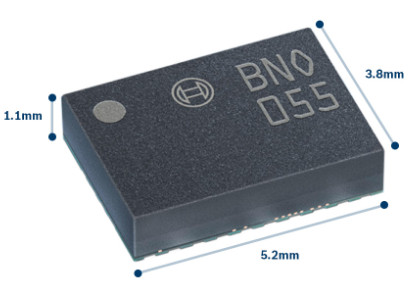
\includegraphics[height=0.5\textwidth]{hardware/bno055.jpeg}
		\caption{Sensor BNO055}
		\label{BNO055}
	\end{subfigure}
	\begin{subfigure}{0.4\textwidth}
		\centering
		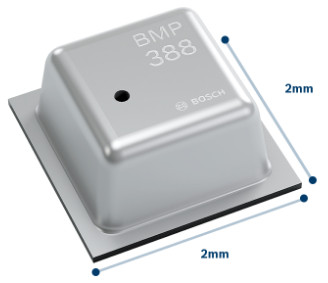
\includegraphics[height=0.5\textwidth]{hardware/bmp388.jpeg}
		\caption{Sensor BMP388}
		\label{BMP388}
	\end{subfigure}
\end{figure}


 
%\section{Otros (Receptora radio)}

\section{Banco de pruebas}
Para poder realizar la experimentación real de forma segura, se han diseñado distintas estructuras para poder sujetar al cuadricóptero permitiéndole rotar con distintos grados de libertad (GdL) en función de la estructura. Estas uniones han permitido poder probar distintos controladores de forma segura y controlada.


Se pueden distinguir 2 tipos de estructuras en función de sus grados de libertad:

\begin{itemize}
	\item \textbf{Rótulas con 1 único grado de libertad}: Para las primeras pruebas de los reguladores es fundamental poder descomponer el control en problemas más sencillos, en este caso permitiendo al sistema rotar en 1 grado de libertad. Se han construido 2 versiones de la misma rótula, una permite el movimiento en Pitch y la otra lo permite en Roll. Esto permite desacoplar los bucles de control y poder probar distintos algoritmos de control.
	
	
	\begin{figure}[htb!]
		\centering
		\begin{subfigure}{0.4\textwidth}
			\centering
			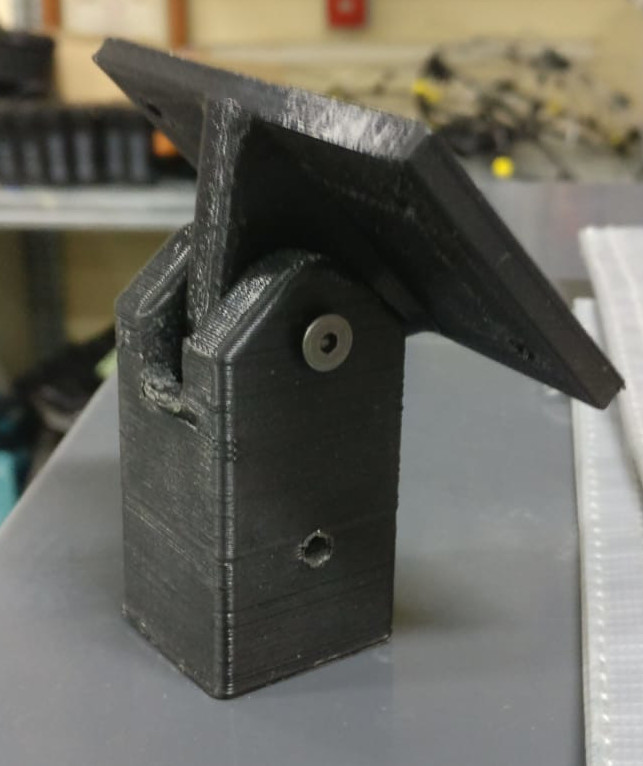
\includegraphics[width=0.8\textwidth,height=0.2\textheight]{hardware/rotulaPitch1.jpeg}
			\caption{Motores LHI MT2204 II empleados}
			\label{a}
		\end{subfigure}
		\begin{subfigure}{0.4\textwidth}
			\centering
			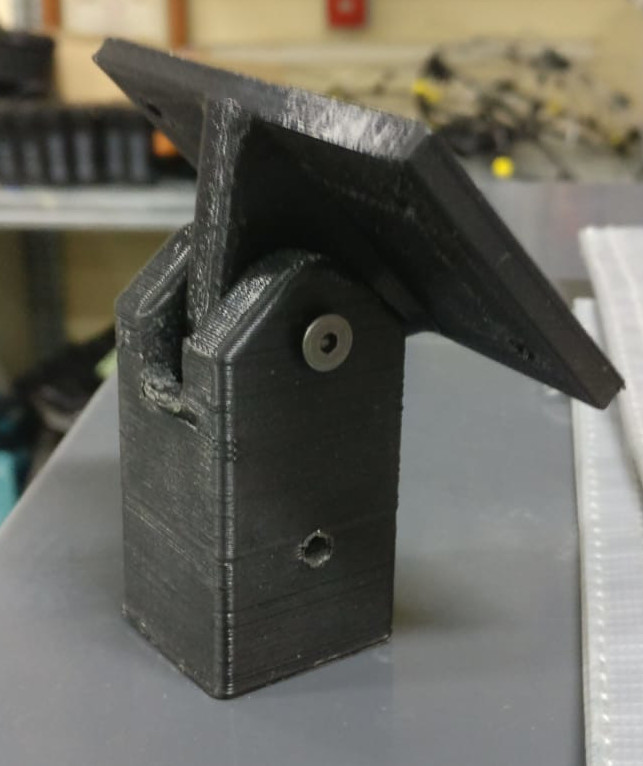
\includegraphics[width=0.8\textwidth,height=0.2\textheight]{hardware/rotulaPitch1.jpeg}
			\caption{ESC Multistar Race 4 in 1 30A BLHeli empleado}
			\label{b}
		\end{subfigure}
	\end{figure}

	Estas uniones son sencillas y robustas lo que nos da seguridad a la hora de poder probar y ajustar los reguladores.
	Las restricciones de movimiento de estas uniones permiten rotaciones de $\pm 60\degree$ en el angulo permitido.
	
	
	\item \textbf{Rótula con múltiples grados de libertad}: Después de conseguir estabilizar al cuadricóptero en pitch y en roll de forma individual la siguiente aproximación consiste en emplear rotulas con 3 GdL. Sobre estas uniones también se han realizado 2 versiones. La primera consta de una única rotula con sus 3 grados de libertad con restricciones de movimiento de:
	
	\begin{align*}
	-60 \degree &\le \varphi \le 60\degree \quad \;\;\;  \text{Roll}\\ 
	-60 \degree&\le \theta \le 60\degree \qquad  \text{Pitch} \\
	-180 \degree&\le \psi \le 180\degree\quad \;  \text{Yaw}
	\end{align*}
	
	
	La segunda consta de acoplar 2 juntas esféricas como las anteriores una a continuación de la otra, lo que permite, además de disminuir las restricciones de movimiento en las rotaciones, pequeños desplazamientos en el espacio tridimensional.
	
	\begin{figure}[htb!]
		\centering
		\begin{subfigure}{0.4\textwidth}
			\centering
			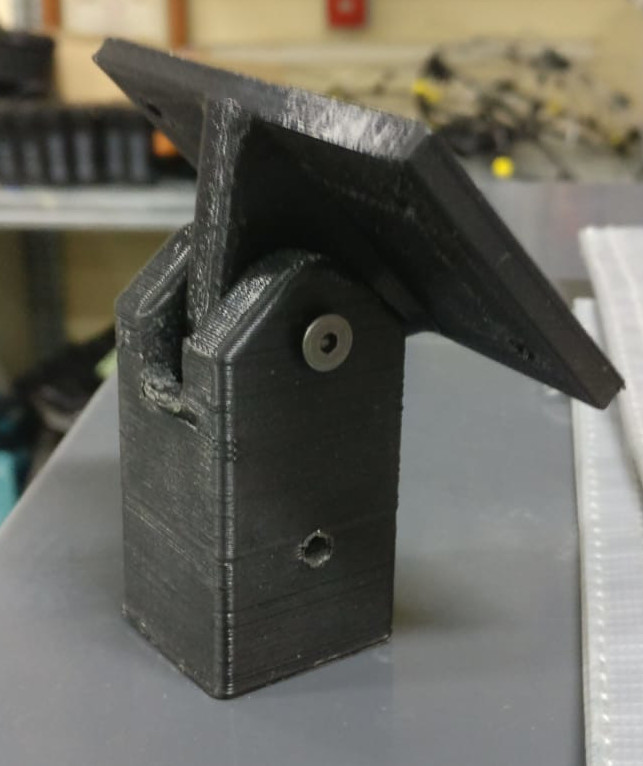
\includegraphics[width=0.8\textwidth,height=0.2\textheight]{hardware/rotulaPitch1.jpeg}
			\caption{Motores LHI MT2204 II empleados}
			\label{c}
		\end{subfigure}
		\begin{subfigure}{0.4\textwidth}
			\centering
			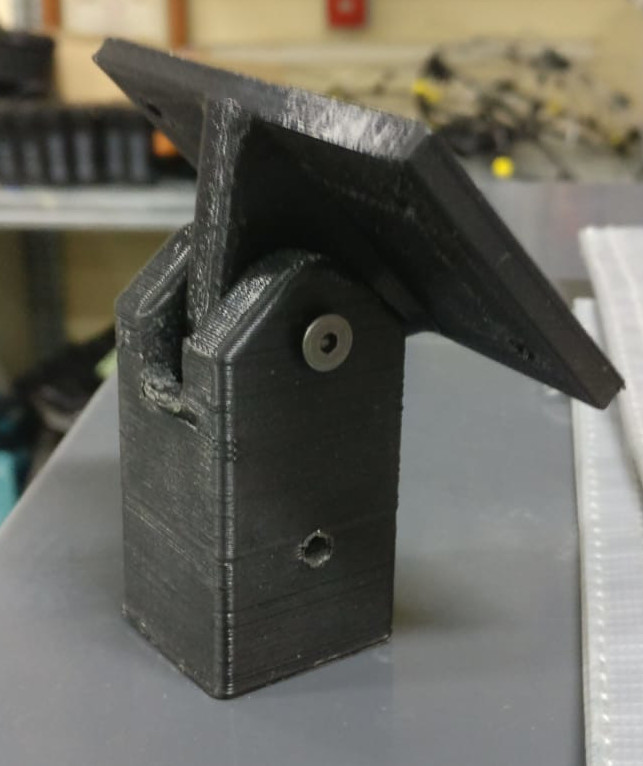
\includegraphics[width=0.8\textwidth,height=0.2\textheight]{hardware/rotulaPitch1.jpeg}
			\caption{ESC Multistar Race 4 in 1 30A BLHeli empleado}
			\label{d}
		\end{subfigure}
	\end{figure}
	
	
	
\end{itemize}


\tb{\huge imagen rotulas y/o CAD }



	\chapter{Software}

Durante el transcurso de este trabajo se ha dividido el desarrollo del software en varias partes, en las cuales se profundizará a continuación.

\section{Software del Autopiloto}
	
	El autopiloto es la parte del multirrotor que se encarga de generar las acciones de control o comandos, que permitan que el dron llegue a un determinado estado.
	Para generar esas acciones de control, el autopiloto estima el estado de la aeronave en cada instante mediante las lecturas de las IMUs y en función del estado genera las acciones de control pertinentes para mantener la estabilidad de la aeronave. Además el autopiloto que se ha desarrollado cuenta con un interfaz WiFi, por lo que permite enviar y recibir datos del autopiloto a una estación de tierra. A continuación se profundizará en como se han llevado a cabo estas tareas.

\subsection{Estimación del Estado}
	Para estimar el estado, el autopiloto toma las medidas procedentes de las 2 IMUs a través del protocolo I2C con una frecuencia de comunicación de 400KHz.
	Las lecturas del BNO055 proporcionan un estado completo de la aeronave con una frecuencia de refresco de 100Hz. Sin embargo, el MPU9250 nos proporciona medidas relativas a las velocidades angulares y aceleraciones lineales con una tasa de refresco más elevada. Es por esto que se han empleado ambos sensores para conseguir el estado deseado con la mayor precisión y menor tasa de refresco posible.
	
	Con este método se consigue estimar el estado deseado:
	 \begin{equation}
	 	S_t=\big(\underbrace{\varphi,\theta,\psi}_\text{BNO} ,\underbrace{\dot\varphi,\dot\theta,\dot\psi}_\text{MPU} \big)
	 \end{equation}
	consiguiendo minimizar la deriva de la estimación, empleando las lecturas muy estables del BNO055, sin perder la reactividad de las medidas que proporciona el MPU9250.
	
\subsection{Interfaz WiFi}
	Con la intención de poder transmitir datos entre el autopiloto y la estación de tierra se ha diseñado un sencillo protocolo de comunicación WiFi basado en el envió de paquetes de tamaño fijo. El ESP32 cuenta con un sistema operativo en tiempo real (RTOS) el cual se encarga de mantener activa las comunicación WiFi de forma transparente al usuario. La estructura de los paquetes es la siguiente:
	
	\begin{itemize}
		\item \textbf{Autopiloto $\rightarrow$ Estación}: Este paquete contiene 6 datos de tipo \textit{float} (32-bits). Se emplea para enviar la estimación del estado a la aeronave en tiempo real. Esto se emplea para tanto monitorización del desempeño de los algoritmos, como para poder cerrar el bucle de control en la estación base y enviar las acciones de control a la aeronave posteriormente. 
		\item \textbf{Autopiloto $\leftarrow$ Estación}: Este paquete contiene 4 datos de tipo \textit{float} (32-bits) y un dato de tipo \textit{byte}. El dato de tipo \textit{byte} se emplea para controlar el modo de funcionamiento de la aeronave, mientras que los otros 4 datos tienen distintos usos en función del modo:
		
		\begin{itemize}
			\item \textbf{MODO 0} (Desarmado): La aeronave se encuentra ``desarmada'' por lo que los motores no reciben acciones de control. En este modo los demás datos del paquete son irrelevantes.
			
			\item \textbf{MODO 1} (\textit{Off-board}): Las acciones de control son emitidas por la estación de tierra, es decir, la aeronave envía la estimación del estado al ordenador y envía el comando recibido a los variadores. En este modo los datos de tipo \textit{float} del paquete representan los comandos de los motores.
			
			\item \textbf{MODO 2} (\textit{On-board}): El algoritmo de control se ejecuta en la aeronave y se generan las señales de control necesarias a una frecuencia  fijada previamente. En el caso de los controladores PID a bordo, los valores de los 4 datos del paquete permiten variar los valores de las constantes del regulador en tiempo real, lo que facilita el ajuste de las mismas.
		\end{itemize}
		
	\end{itemize}

\subsection{Generacion de comandos \textit{on-board}}
	Para poder maximizar la frecuencia del algoritmo de control y permitir el control de la aeronave sin necesidad de una estación de tierra, los algoritmos de control validados en la simulación se pueden implementar directamente en el autopiloto, fijando previamente la frecuencia a la que se desea que se ejecute el algoritmo. 
	\tb{actualizar en el momento}
	En este trabajo se han implementado a bordo dos algoritmos de control distintos: un regulador PID clásico y un regulador PID en cascada.
	
\section{Software de la estación}

La estación base se ha empleado tanto como para la simulación del entorno, permitiendo diseñar y probar algoritmos de control de forma segura, como para monitorizar los rendimientos de estos algoritmos o incluso, aprovechando la mayor capacidad computacional de estas estaciones, ejecutar los algoritmos de control y aprendizaje por refuerzo en estas.
A continuación se profundizará con más detalle en la implementación de estas herramientas. 


\subsection{Entorno de simulación}

En cualquier proyecto de robótica es conveniente contar con un entorno de simulación que permita realizar pruebas en distintas situación de forma sencilla y rápida, sin necesidad de tener ni modelo real, ni el entorno concreto en el que quieras probar tu robot. Cuando se trabaja con drones, la simulación pasa de ser conveniente a ser muy necesaria. Ésto es debido a la peligrosidad intrínseca de estas aeronaves, ya que, cuentan con hélices que giran a gran velocidad.

%Es por esto que es necesario contar con un entorno de simulación en el que se puedan probar los algoritmos de control antes de llevarlos a la realidad, con el objetivo de minimizar los riesgos de estas pruebas.Si a todo esto se le añade la experimentación con algoritmos de aprendizaje por refuerzo e inteligencia artificial, la simulación y entrenamiento previos se hacen imprescindibles 

Debido a la naturaleza del apredizaje por refuerzo, este requiere de la interacción de un agente con un entorno para que el agente aprenda que acciones son las que debe tomar en cada estado. Esto significa que al comienzo del entrenamiento el agente realiza acciones aleatorias para poder explorar cuales son las que le proporcionan una recompensa mayor.

Debido a esta forma de explorar, el agente requiere de una gran cantidad de pruebas, de ensayo y error, hasta que consigue aprender, por lo que no es conveniente realizar todas estas iteraciones en un modelo real.

Por estas razones se necesita de un entorno de simulación para poder validar los algoritmos y poder generar modelos entrenados en simulación sin deteriorar el equipo real. Además el entorno en simulación te permite entrenar distintos agentes simultáneamente y reducir los tiempos de entrenamiento.

Para el entorno de simulación nos hemos basado en Gym \tb{citar},una librería escrita en Python y desarrollada por la compañía OpenAI, que permite desarrollar y comparar algoritmos de aprendizaje por refuerzo. Esta librería te permite generar un entorno con el cual interactúe el agente, sin importar la implementación de éste, permitiendo comparar el rendimiento de distintos agentes sobre el mismo entorno.
\tb{IMAGEN GYM}

\tb{revisar} Como entorno de simulación se ha partido de GymFC, desarrollado por William Koch et al. \cite{koch2019reinforcement}.
Este entorno de simulación utiliza Gazebo 9, un entorno de simulación 3D de código abierto ampliamente utilizado en el campo de la robótica. En este entorno se simula el comportamiento de un multirrotor, concretamente el de un modelo del cuadricóptero IRIS.
\tb{imagen GYMFC}

Para acercar la simulación a la configuración de los experimentos que se realizarían posteriormente en la plataforma real, se han realizado algunas modificaciones sobre el modelo predeterminado de la aeronave:

\begin{enumerate}
	\item Se ha modificado la forma de anclaje del cuadricóptero. Originalmente el dron se encontraba anclado entorno a una articulación situada en su centro de gravedad. Esto permitía que el peso de la aeronave apenas tuviera influencia a la hora de rotar la aeronave, todo el peso estaba sustentado por la articulación, lo cual no se asemeja con los bancos de pruebas que se han diseñado. En estos bancos de prueba el anclaje se encuentra desplazado con respecto al centro de gravedad, por lo que cuanto mayor sea el valor de los ángulos $\varphi$ y $\theta$ mayor es la influencia del peso en el par necesario para estabilizar la aeronave. Es por esto que se ha desplazado la articulación del centro de gravedad y se ha conectado a la aeronave mediante una unión rígida, asemejando así el entorno de simulación al entorno de pruebas real.
	\item Se ha modificado parámetros dinámicos de la aeronave. Los parámetros que mayor discrepancia tenían entre la simulación y el mundo real eran principalmente los parámetros inerciales. Tanto la masa como los momentos de inercia del cuadricóptero eran mucho inferiores a los de la aeronave real. Esto se manifestaba principalmente cuando al hacer pruebas con los algoritmos PID el comportamiento simulado no se parecía con el real, por ejemplo en simulación un regulador P era capaz de estabilizar al sistema, mientras que en la realidad un regulador P era inestable de por sí y requería de las acciones derivativa e integral para conseguir estabilizarlo.
\end{enumerate}

%Para acercar la simulación a la configuración de los experimentos que se realizarían posteriormente en la plataforma real, se ha situado una articulación en su centro de gravedad que fija la posición de su centro pero permite rotar el numero de grados de libertad que se predefina.


 \subsection{Agente (generación de comandos)}
 
 Siguiendo con la terminología del aprendizaje por refuerzo se va a denominar agente al encargado de generar las acciones de control. Dependiendo del algoritmo de control que se use, se dispone de distintos tipos de agente.
 
 \subsubsection{Agente con algoritmos PID}
 En este caso, el agente recibe las observaciones del entorno a través del estado y en función de éste, produce la salida a los motores. Este agente es el más sencillo, ya que , una vez ajustadas las ganancias, éste solamente debe enviar los comandos de control a la aeronave.
 
 \subsubsection{Agente con algoritmos de RL}
 Este agente, se encarga, tanto de generar las acciones como de optimizar la política que las genera.
 
 
 El agente, basado en el estado observado $s_t$ y la política $\pi$ actual, genera una acción $a_t$, tras realizarla, el entorno le proporciona un estado $s_{t+1}$ y una recompensa $r_t$.
 Con esta tupla $[s_t,a_t,r_t,s_{t+1}]$ el agente emplea el algoritmo de aprendizaje por refuerzo definido para actualizar la política $\pi$ y así intentar mejorarla con cada iteración. 

Para probar distintos distintos algoritmos se han empleado la implementación de los algoritmos del estado del arte, del repositorio de GitHub \textit{Stable-Baselines} \cite{stable-baselines}. Inicialmente se comenzó empleando las \textit{Baselines} de OpenAI \cite{OpenAIbaselines} pero se decidió cambiar a las \textit{Stable Baselines} por la limpieza del código y la facilidad para realizar experimentos con diversos algoritmos e hiperparámetros. Con esta herramienta se ha podido experimentar con distintos algoritmos para comparar el rendimiento conseguido de cada uno.


\subsection{Interfaz Estación-Autopiloto}

Para las pruebas reales se ha empleado ROS (Robotic Operative System) Melodic para gestionar la comunicación WiFi con la aeronave y la comunicación con el agente. Para esto se emplea la estructura de \textit{topics}: un \textit{topic} se emplea para enviar datos a la aeronave y otro \textit{topic} publica los datos recibidos por ésta. De esta manera se pueden utilizar las herramientas de ROS para poder monitorizar el proceso además de aprovechar la estructura de \textit{topics} para poder intregrar código escrito en distintos lenguajes de forma sencilla.

\begin{figure}[htb!]
	\centering
	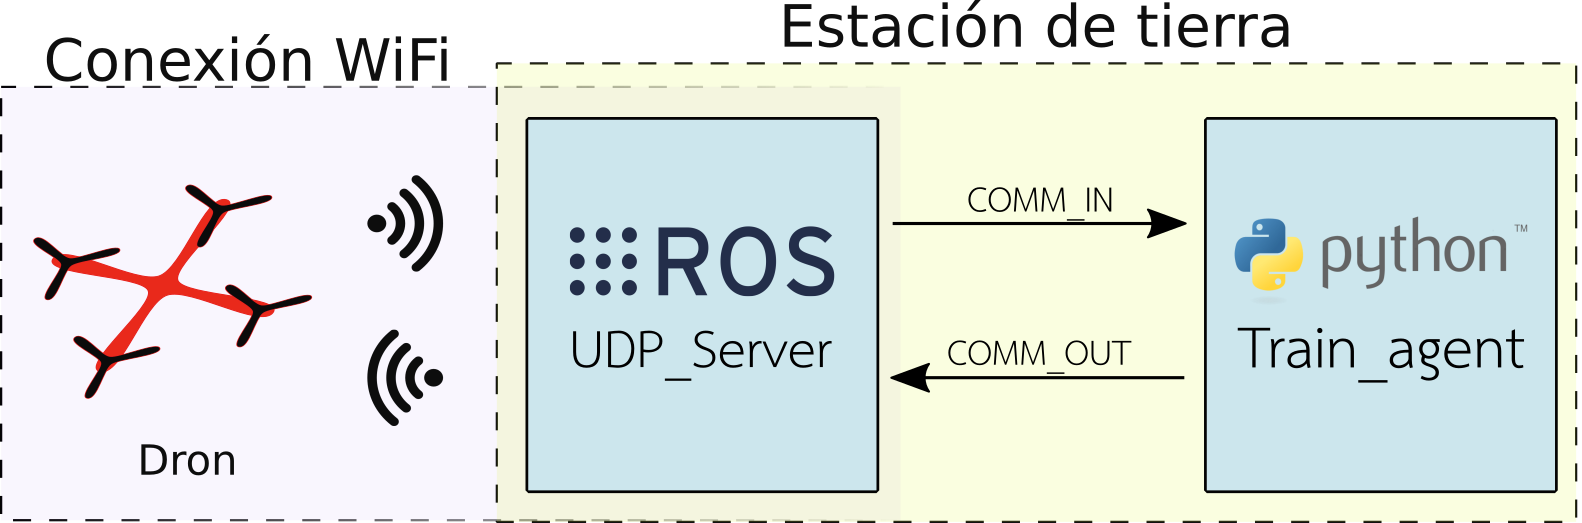
\includegraphics[width=0.9\textwidth]{software/Arquitectura}
	\caption{Esquema interfaz Estacion-Autopiloto}
	\label{hardware:esc_explicacion}
\end{figure}





\section{Descripción del equipo}
Para el desarrollo del trabajo se ha empleado un portatil MSI-GE62 empleando Windows 10 para el desarrollo CAD y Ubuntu 18.04 LTS para el resto de las tareas. El equipo cuenta con 16GB de RAM DDR4, un procesador Intel i7-6700HQ de 8 núcleos a 2.60GHz y una GPU GeForce GTX 970M con 3GB de memoria dedicada.


	\chapter{Metodología (\tb{Problem Formulation})}

El objetivo del trabajo es estabilizar un UAV usando algoritmos de control basados en una red neuronal entrenada empleando algoritmos de aprendizaje automático. Los principales componentes que intervienen en el agente son el estado, las acciones y la recompensa, para cada problema hay un conjunto que estados, acciones y funciones de recompensa que pueden llevar a que el agente aprenda.

\section{Diseño del estado}
 El autopiloto cuenta con 2 IMUs para poder obtener datos sobre su estado. Se quiere estabilizar el dron en una orientación concreta, por lo tanto el estado que se ha diseñado consta de 6 parámetros:
\begin{equation}
	S=(\varphi,\theta,\psi,\dot\varphi,\dot\theta,\dot\psi) \qquad\qquad \varphi,\theta,\psi,\dot\varphi,\dot\theta,\dot\psi \in [-1,1]
\end{equation} 

Siendo $\varphi,\theta$ y $\psi$ los ángulos de alabeo (\textit{roll}), cabezeo (\textit{pitch}) y guiñada (\textit{yaw}) del dron  y $\dot\varphi,\dot\theta$ y $\dot\psi$ sus respectivas velocidades. Para favorecer la convergencia del aprendizaje, se ha normalizado el estado para que todas sus componentes estén comprendidas dentro del intervalo $[-1,1]$.

Los ángulos proporcionan información sobre el estado actual y la velocidad angular sobre los estados pasados, es decir, proporciona cierta información temporal. 

Para obtener la estimación de orientación se han fusionado las medidas de las 2 IMUs del autopiloto utilizando un filtro complementario, para así conseguir una buena estimación estática junto con una buena respuesta dinámica.
\section{Diseño de las acciones}
Al trabajar con un quadricóptero podemos actuar sobre la potencia que se le entrega a los motores, por lo que cada acción que realice el agente constará de 4 campos:
\begin{equation}
	A = (T_1,T_2,T_3,T_4) \qquad\qquad T_i \in [-1,1]
\end{equation}
Siendo $T_i$ la potencia \textit{(Thrust)} normalizada entregada a cada motor. Un valor de $T_1=-1$ significa que el motor 1 estaría girando a la mínima potencia permitida y un valor de $T_1=1$ corresponde a que el motor 1 estaría girando a la máxima potencia.\\

\tb{\huge completar con la transformacion del mundo -1,1 al mundo 1000,2200 $\mu S$}

\section{Diseño de la función de recompensa}
La función de recompensa rige la forma en la que la red va a configurar sus pesos, por lo tanto, cómo se va a comportar el agente en un estado determinado.
Para conseguir que el agente responda de la forma deseada se han probado una gran variedad de funciones de \textit{reward}, optando finalmente por:
\begin{equation}
	%R_t = \left( 1-\frac{|\varphi - \varphi_{ref}| + |\theta-\theta_{ref}| + |\psi- \psi_{ref}|}{3}\right)^3
	R_t = \left( 1-\frac{|\varphi|  + |\theta| + |\psi|}{3}\right)^3
\end{equation}
Con esta funcion de recompensa \tb{BLA BLA BLA}


	\chapter{Experimentos}
Pa
	\chapter{Discusión}
	\chapter{Conclusiones y trabajo futuro}

Durante el transcurso de este proyecto se ha conseguido desarrollar una plataforma, que permite estudiar los distintos algoritmos de control, con los que se puede estabilizar a un cuadricóptero. A continuación se hablara sobre las conclusiones que se han extraído durante este proceso y las posibles líneas de mejora que se podrían realizar en un futuro. En los apéndices se encuentra la planificación , el presupuesto y el impacto medioambiental del trabajo. 

\section{Conclusiones}

Los objetivos principales que se plantearon al comienzo del proyecto consistían en: desarrollar un autopiloto propio capaz de ejecutar distintos algoritmos de control para cuadricópteros, desarrollar una plataforma de vuelo para poder probar este autopiloto y los algoritmos de forma segura e investigar sobre la posibilidad de emplear distintos algoritmos de aprendizaje por refuerzo para el control de actitud de la aeronave. A continuación desgranaremos las conclusiones que se han extraído de cada uno de estos objetivos y las posibles mejoras que se pueden realizar de cada uno.

\subsubsection{Autopiloto}
Se ha conseguido desarrollar un autopiloto funcional, capaz de estimar el estado de la aeronave y estabilizarse, cerrando un bucle interno de control y generando los comandos necesarios para controlar los motores. En este autopiloto se ha integrado la etapa de potencia necesaria para que sea posible alimentar al mismo directamente desde la batería, por lo que integra en una única PCB una gran cantidad de funcionalidades que no son habituales en los autopilotos comerciales, como por ejemplo la conexión WiFi, lo que ha permitido recabar los datos en tiempo real de forma sencilla. Sin embargo, las pistas que alimentan los motores a través de placa no se encuentran lo suficientemente ventiladas, por lo que se calientan demasiado.

\subsubsection{Plataforma de vuelo}
La plataforma de vuelo, ha permitido llevar a cabo los experimentos realizados de una forma segura y controlada. Debido a que la inmensa mayoría de las piezas han sido fabricadas mediante técnicas de impresión 3D, ha sido posible realizar variaciones de la plataforma de forma rápida y sencilla. Es por ésto que ,  se han diseñado varios componentes intercambiables, para poder modificar la configuración de los experimentos, lo que ha sido crucial para poder realizar el ajuste los parámetros del PID en las pruebas reales. El inconveniente que tiene la impresión 3D empleando PLA, es la fragilidad de algunas piezas, como por ejemplo, la unión esférica del banco de pruebas.

\subsubsection{Algoritmos basados en aprendizaje por refuerzo}

Uno de los retos que más tiempo han requerido, ha sido conseguir que los algoritmos propuestos, convergieran a una política óptima. Ha sido un proceso iterativo que ha tomado mucho tiempo hasta que se consiguió la convergencia del primer algoritmo. Posteriormente se realizaron muchas modificaciones de los hiperparámetros con el ánimo de mejorar el comportamiento del agente. Finalmente se ha conseguido aplicar varios algoritmos del estado del arte, consiguiendo , en algunos casos como en el del TRPO, muy buenos rendimientos.

\section{Trabajo futuro}

Esta plataforma, puede tener un gran interés para labores investigadoras y docentes. Para que pueda ser empleable de forma cómoda en estos ámbitos, sería posible simplificar el autopiloto, reduciendo así su tamaño y coste, ademas de reducir las dimensiones de la aeronave y el banco de pruebas, empleando por ejemplo motores DC, los cuales son mucho más pequeños y permiten controlarse de forma más sencilla. Si se reduce el tamaño, sería posible emplear varias de estas plataformas en los laboratorios de institutos y universidades para enseñar teoría de control. Además de reducir el tamaño, sería conveniente diseñar un interfaz más sencillo, pudiéndose integrar con programas como Matlab y Simulink, ésto mejoraría la usabilidad del mismo.

De cara a la investigación, sería conveniente realizar un modelo preciso de la aeronave en concreto, en vez de usar el modelo de otro cuadricóptero. Cuanto más parecido sea el modelo que se emplea en simulación al modelo real de la aeronave, menos se diferenciarán los comportamientos observados en simulación y el comportamiento real. En el desarrollo de algoritmos basados en aprendizaje por refuerzo, un aspecto muy relevante es el salto entre el entorno simulado y el entorno real, si el modelo real es lo suficientemente distinto al simulado, los comportamientos pueden variar enormemente. Es por esto que sería conveniente realizar una modelización dinámica completa de la aeronave.

En cuanto a los algoritmos, existen muchas maneras distintas de poder emplear el aprendizaje automático al campo del control de cuadricópteros, sería interesante replantearse la forma en la que los algoritmos actúan, para mejorar el rendimiento de estos algoritmos de forma que sobrepasen a los algoritmos de control clásico.Por ejemplo, en vez de generar un controlador en posición basado en RL, sería interesante diseñar un controlador en velocidad y sobre éste emplear un regulador P, basándose en la filosofía del controlador en cascada.  







	
	
	\appendix
\chapter {Esquemáticos del autopiloto}
A continuación se adjuntan los esquemáticos del autopiloto diseñado.

\begin{figure}[htb!]
	\centering
	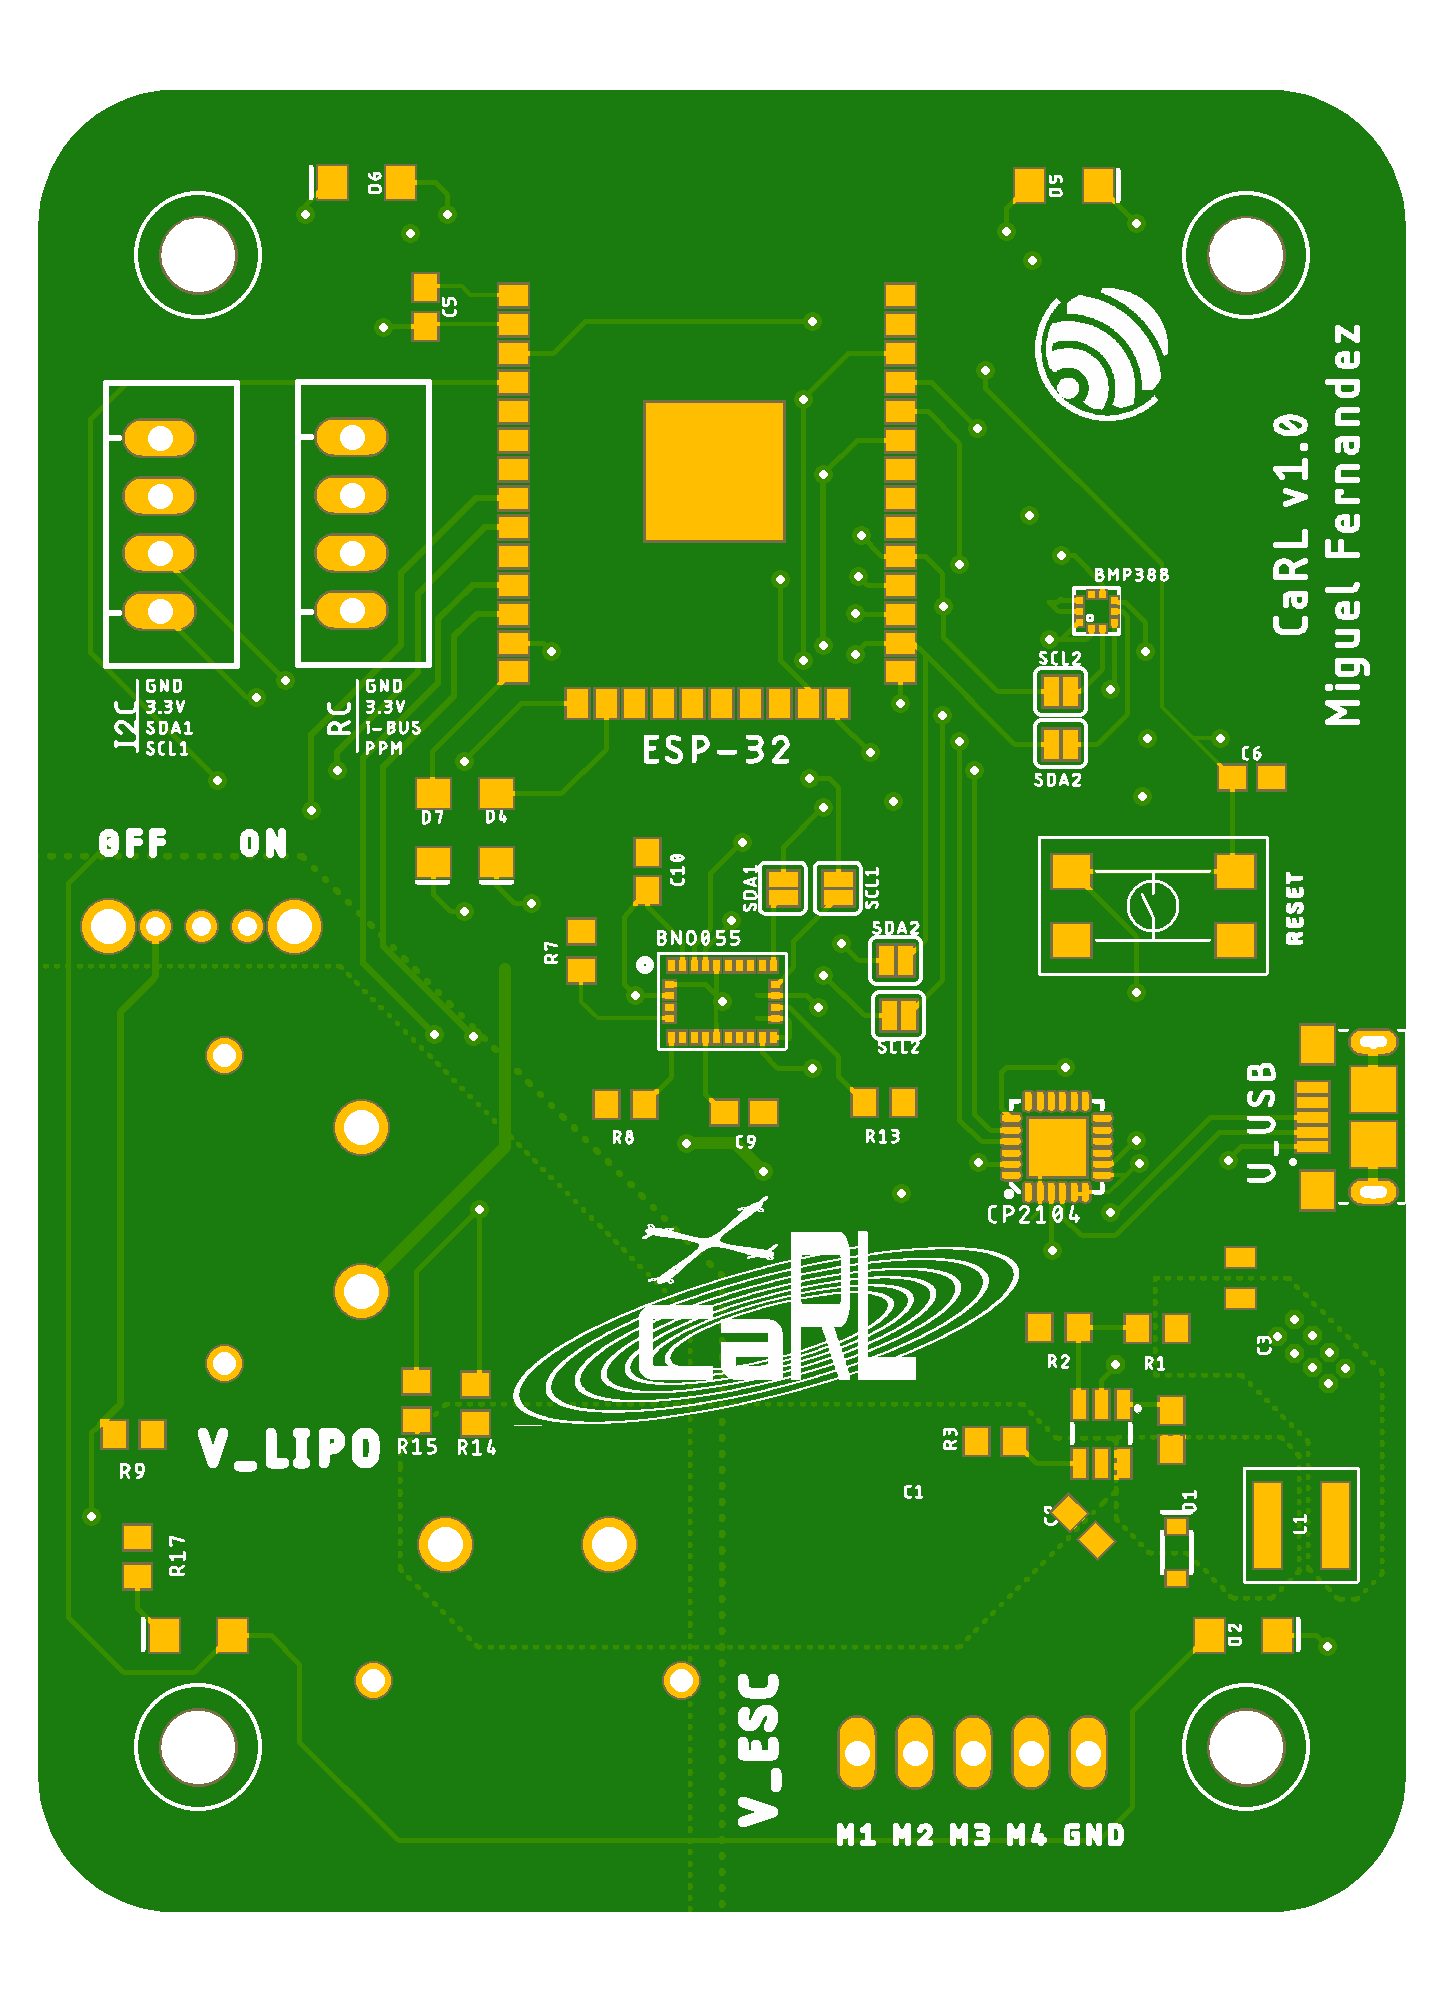
\includegraphics[height=0.7\textheight]{CaRLv1}
	\caption{\textit{Board} PCB Autopiloto.}
	\label{gantt}	
\end{figure}

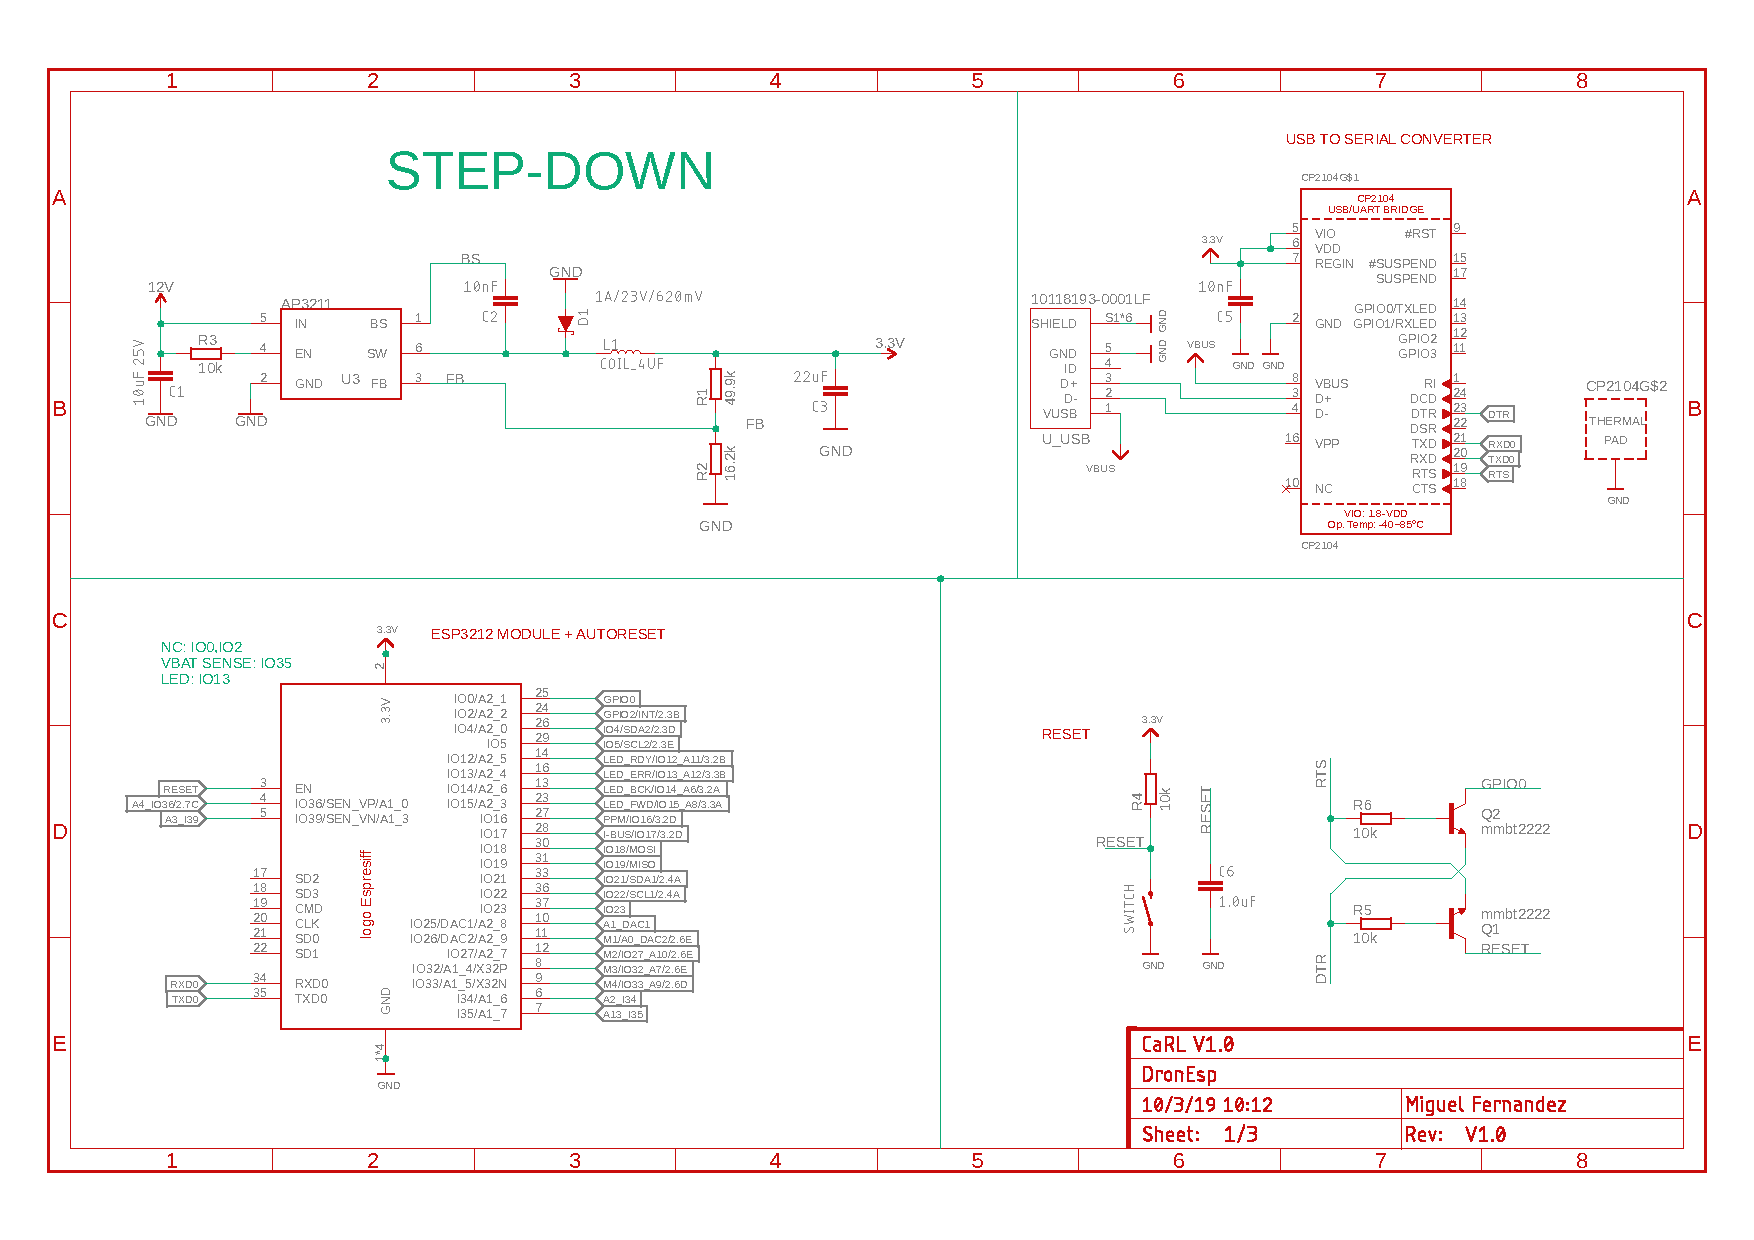
\includepdf[pages=-,angle=90]{DronEsp.pdf}
 
\chapter{Presupuesto y Planificación}
\section{Presupuesto}

El presupuesto del trabajo se puede separar en tres partes: recursos humanos, compra de material y amortización de los equipos utilizados.

En cuanto a los recursos humanos empleados, se ha tenido una dedicación por parte del alumno de unas 800 horas, esto es un número de horas mucho superior a las 360 horas (30h/ECTS) correspondientes a la carga temporal de los 12 ECTS del Trabajo fin de Grado (TFG). Esto se ha debido al gran alcance y a la complejidad del mismo. Un sueldo de investigador a media jornada en la universidad, sin estar graduado, es de unos 450 euros. Lo que se traduce en un salario de unos 5,625 euros la hora. Los salarios del tutor y el cotutor se han extraído del portal de transparencia de la UPM. La dedicación del tutor ha sido de unas 20 horas de implicación en el trabajo y la implicación del cotutor ha sido de unas 80 horas de implicación.  

\begin{figure}[htb!]
		\centering
		\begin{tabular}{|l|r|r|r|}
		\hline
		%\textbf{Recursos humanos} &Coste unitario [EUR] &Unidades&Total [EUR]\\
		
		\textbf{Recursos humanos} & Horas &Coste Horario [EUR]&Total [EUR]\\
		\hline
		
		Alumno & 800 & 5.625 &  4500 \\
		Cotutor & 80 & 7.8 & 624\\
		Tutor & 20& 33.72 & 674.4 \\
		\hline
		\textbf{Total} & &  & \textbf{5798.4}\\
		\hline
		\end{tabular}\\
	
\end{figure}

Los costes de material del proyecto son debidos a la construcción del cuadricóptero y del autopiloto.


\begin{figure}[htb!]
	\centering
	\begin{tabular}{|l|r|r|r|}
		\hline
		\textbf{Material} &Coste unitario [EUR] &Unidades&Total [EUR]\\
		
		\hline
		
		\textbf{Cuadrcóptero}& & &  \\
		Bobina PLA 1Kg & 20 & 1.5 &  30 \\
		Perfiles aluminio & 2 & 1 & 2\\
		Pack 4 Motores MT2204 II & 25 &1& 25 \\
		ESC BlHeli 4 in 1  & 50 & 1 & 50\\
		Baterías LiPo & 25 & 2 & 50\\
		PCB autopiloto & 20 & 1 & 20\\
		Componentes PCB & 50 & 1  & 50 \\
		Hélices HQ5040 &2.5&4&10\\
		\hline
		\textbf{Total} & &  & \textbf{239}\\
		\hline
	\end{tabular}\\
\end{figure}

En cuanto a la amortización del equipo, se han empleado 2 ordenadores para el desarrollo del software y para el entrenamiento de los algoritmos. Se ha considerado una amortización lineal del 10 \% de la vida útil (10 años).

\begin{figure}[htb!]
	\centering
	\begin{tabular}{|l|r|r|r|}
		\hline
		\textbf{Equipo} & Precio &Coste Amortización(10\%)\\
		\hline
		
		Pc sobremesa & 1980 & 198\\
		Pc portátil & 1300 & 130\\
		\hline
		\textbf{Total} & & \textbf{328}\\
		\hline
\end{tabular}\\
\end{figure}

Añadiendo un coste de encuadernado de la memoria de unos 30 euros el presupuesto total del proyecto ha sido



\begin{figure}[htb!]
	\centering
	\begin{tabular}{|l|r|r|r|}
		\hline
		\textbf{Concepto} &Total [EUR]\\
		\hline
		Recursos humanos & 5798.4\\
		Material &239\\
		Amortización del equipo & 328\\
		Encuadernación&40\\
		
		\hline
		\textbf{Total}   & \textbf{6405,4}\\
		\hline
	\end{tabular}\\
\end{figure}





\section{Planificación}
La realización de este trabajo ha empleado un ritmo continuo de horas de trabajo desde su comienzo, siendo un poco menor en épocas de exámenes y un poco mayor al comienzo de los cuatrimestres y julio. La dedicación media diaria del trabajo ha sido de unas 4 horas semanales, durante un periodo de unos 10 meses (descontando agosto y septiembre), lo que da un total de unas 800 horas. La inmensa mayoría de estas horas se han dedicado en el Centro de Automática y Robótica (CAR) de la Escuela Técnica Superior de Ingenieros Industriales (ETSII) de la Universidad Politécnica de Madrid (UPM), concretamente en el grupo de investigación de Visión por Computador y Robots Aéreos (CVAR).

En cuanto a la distribución del trabajo en este tiempo, el trabajo comenzó a realizarse en septiembre de 2018, durante los primeros meses se realizó el curso sobre redes neuronales y aprendizaje profundo, en la plataforma online Coursera. La duración del curso se extendió hasta finales de diciembre. Paralelamente, a partir de octubre se comenzó con el diseño de la aeronave, y en noviembre con el del autopiloto. A principios de febrero se finalizo con el diseño y construcción del cuadricóptero y con el diseño y montaje de la PCB del autopiloto. A partir de este punto, el resto del tiempo se ha dedicado al software, tanto el del autopiloto, como el de la estación de tierra , al diseño de los algoritmos de control y a la experimentación real. Se ha realizado un diagrama GANTT (\cref{gantt}) en el que se ha detallado más en profundidad la distribución temporal de las tareas. Asimismo, se ha esquematizado la organización del proyecto en un diagrama EDP (\cref{EDP}). 

\begin{figure}[htb!]
	\centering
	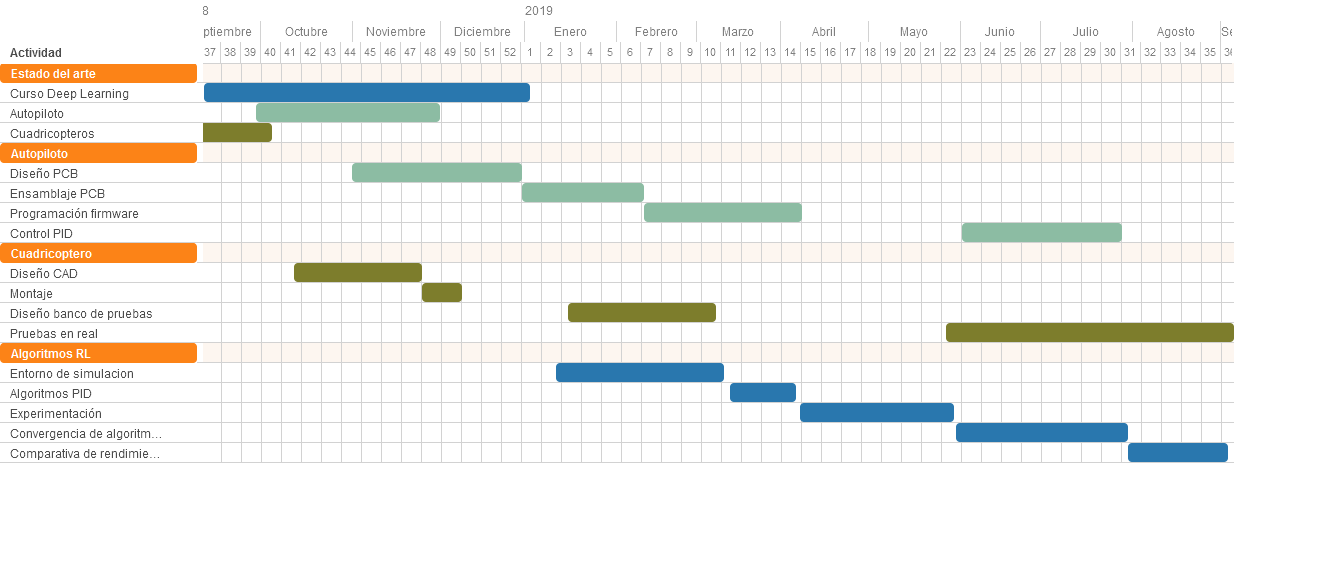
\includegraphics[width=\textwidth]{planificacion_ambiental/gantt}
	\caption{Diagrama de Gantt}
	\label{gantt}	
\end{figure}

\begin{figure}[htb!]
	\centering
	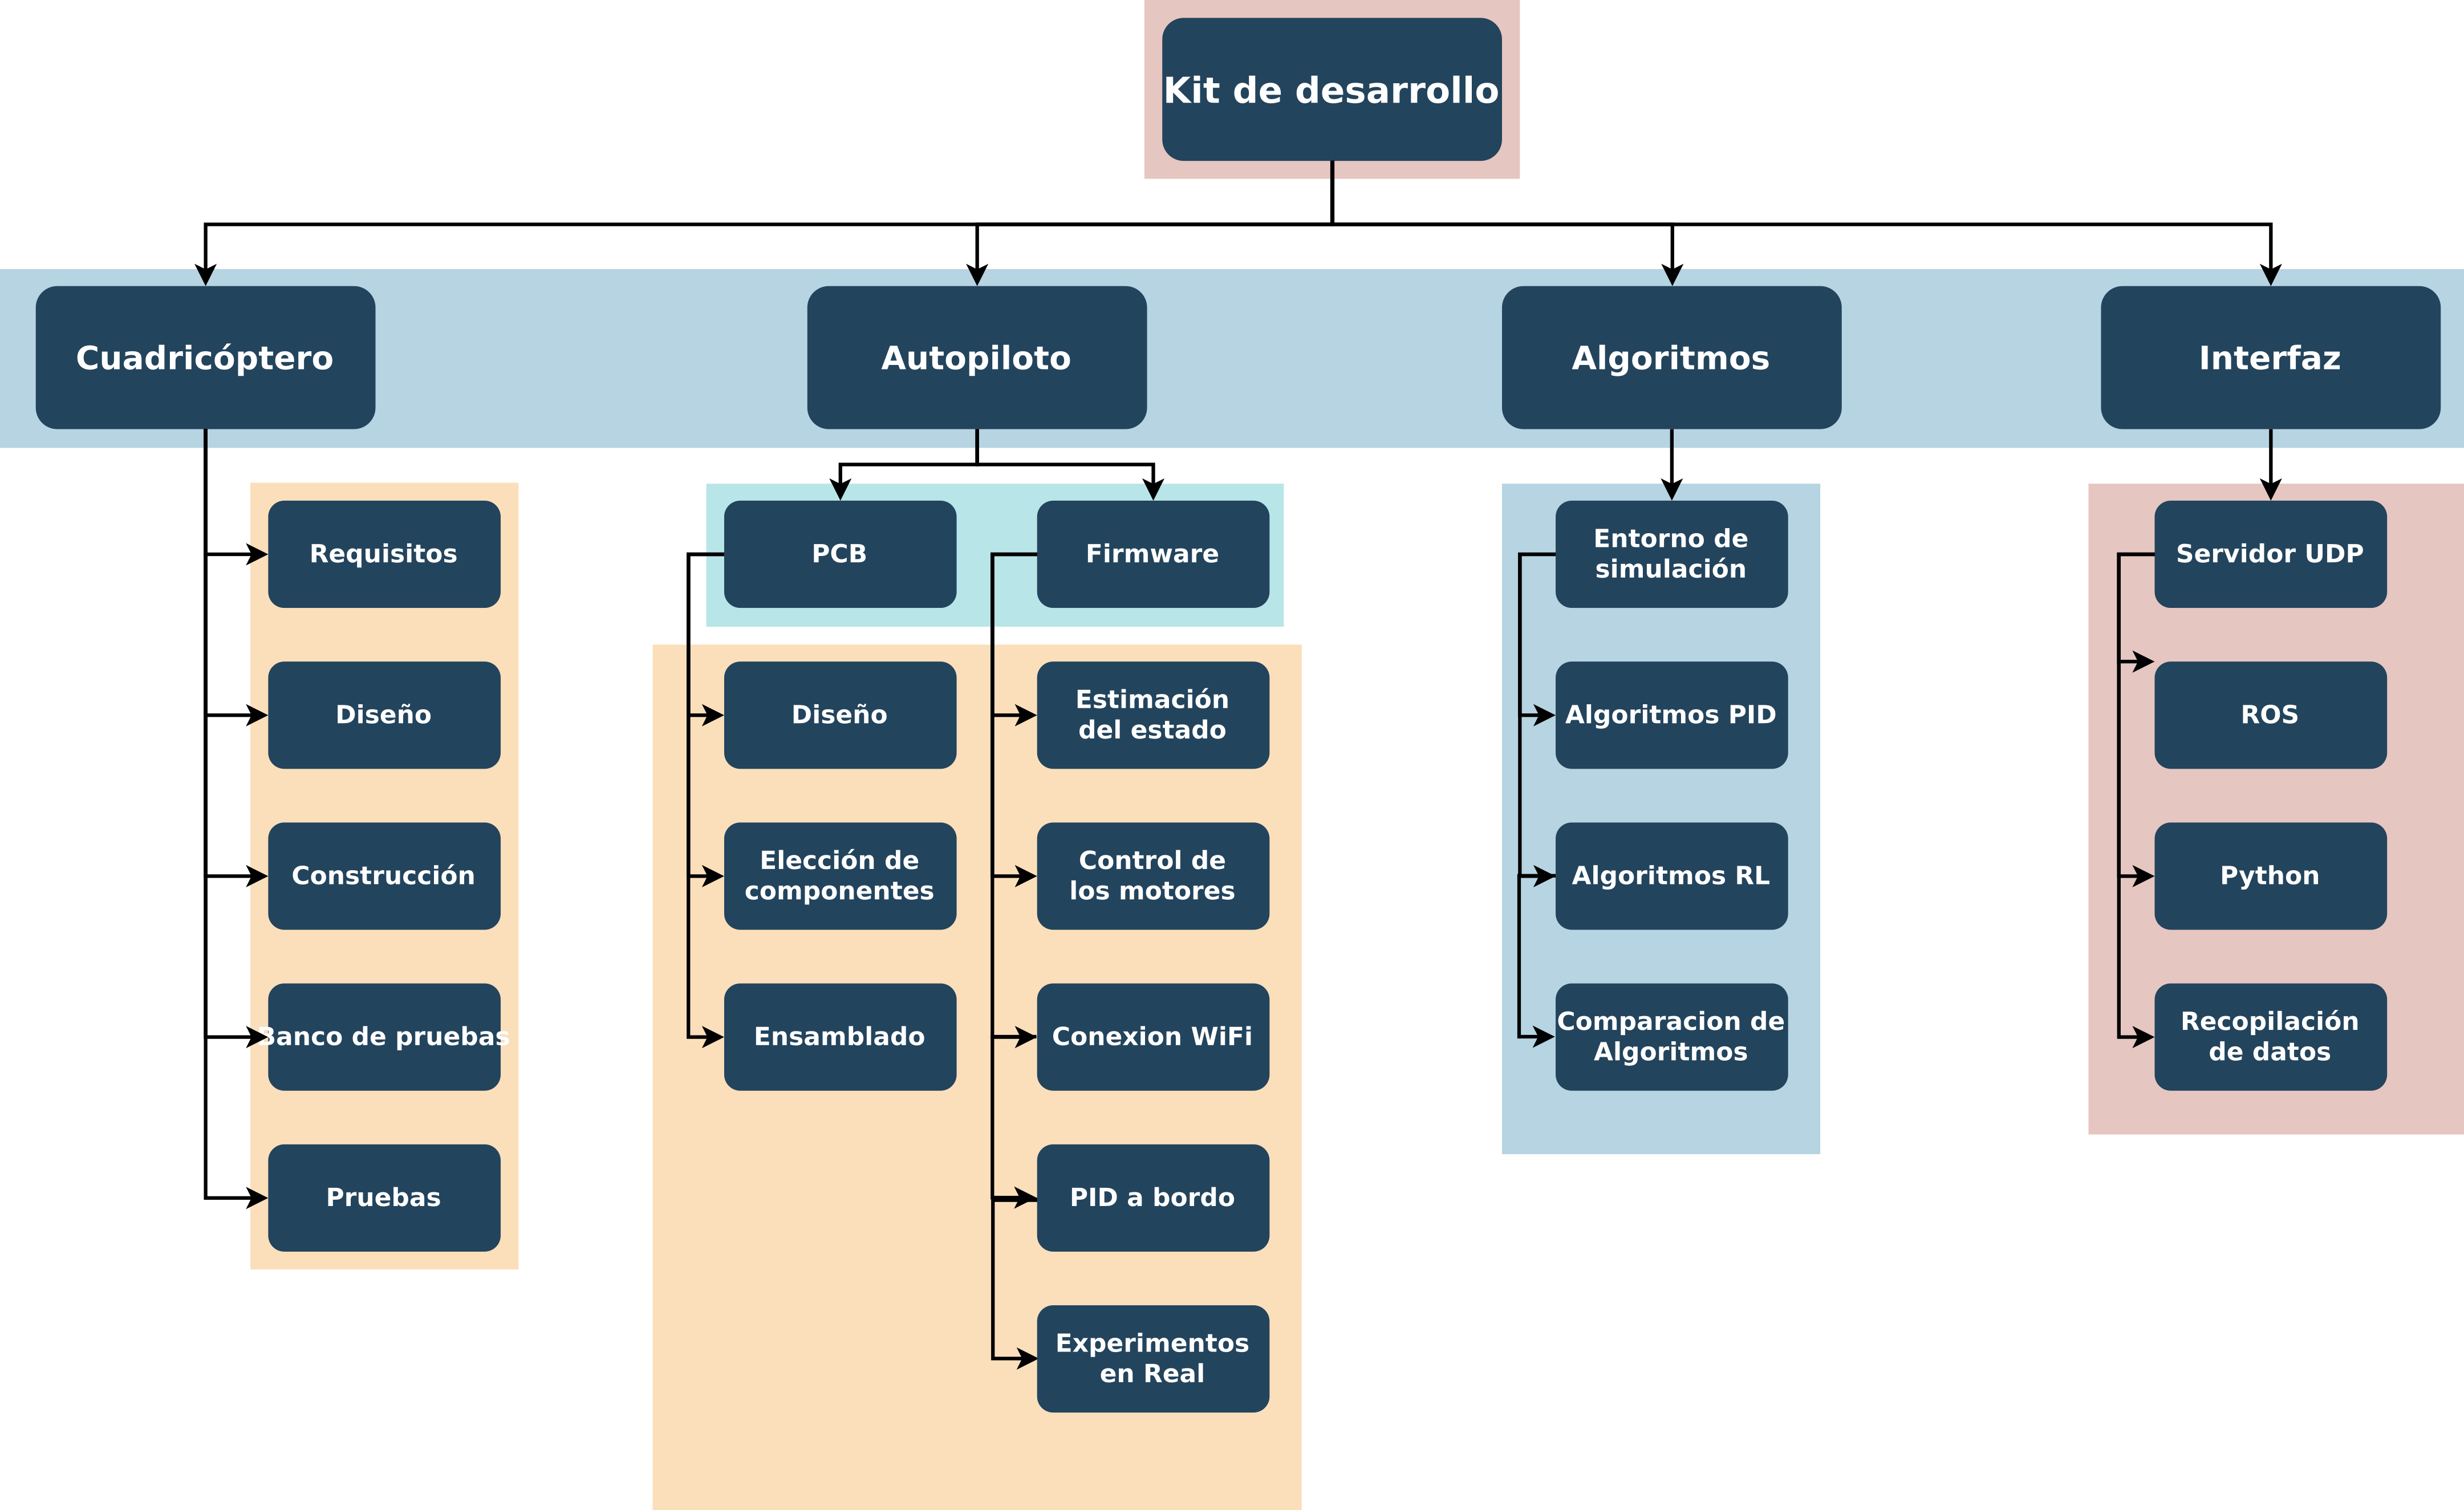
\includegraphics[width=\textwidth]{planificacion_ambiental/edp}
	\caption{Diagrama EDP}
	\label{EDP}	
\end{figure}



\chapter{Impacto social y medioambiental}

El impacto social que tiene este trabajo se ve reflejado en su posible empleo en la educación y la investigación. Actualmente las metodologías docentes están tendiendo hacia el aprendizaje práctico, hacia aprender haciendo. Esta plataforma podría emplearse en centros docentes debido a su montaje mecánico hecho casi en su totalidad con impresión 3D.

Desde el punto de vista de la investigación, tener la posibilidad de desarrollar y probar nuevos algoritmos para el control de cuadricópteros puede mejorar la efectividad del uso de estas aeronaves en múltiples aplicaciones. Cuanto mejor sea el controlador, más fácil será utilizar estas aeronaves para tareas de inspección, seguridad y búsqueda y rescate, entre otras.

El impacto medioambiental de la plataforma es reducido, ya que, el PLA es un plástico biodegradable y las baterías de Litio, una vez descargadas, son sencillas de desechar. EL proceso de fabricación de los componentes requiere de recursos materiales y energéticos, cuyo proceso de obtención  puede provenir de fuentes no renovables. Sin embargo, los beneficios sociales que se pueden extraer de los resultados del proyecto hacen asumible este impacto medioambiental.



	\newpage
	\cfoot{\thepage}
	\pagenumbering{arabic}
	
	\listoffigures
	\listoftables
	\nocite{*}
	\bibliographystyle{IEEEtran}
	\bibliography{IEEEabrv,workBibliography}
	
\end{document}
